% =====================================================================
%  Training a GPT-Style Language Model from Scratch
%  Pratik Ramdas Sonawane -- Vizuara Technologies
%  Compile with pdfLaTeX (Overleaf default). Red [ ... ] marks values to fill in.
% =====================================================================
\documentclass[11pt,a4paper]{article}

\usepackage{iftex}
\ifPDFTeX
  \usepackage[T1]{fontenc}
  \usepackage[utf8]{inputenc}
  \usepackage{lmodern}
\else
  \usepackage{fontspec}
\fi
\usepackage[a4paper,margin=2.5cm]{geometry}
\usepackage{microtype}
\usepackage{amsmath,amssymb}
\usepackage{graphicx}
\usepackage{booktabs,longtable,tabularx,array}
\usepackage{caption}
\usepackage{subcaption}
\usepackage{xcolor}
\usepackage{enumitem}
\usepackage{listings}
\usepackage{pdflscape}
\usepackage[colorlinks=true,linkcolor=blue!50!black,citecolor=blue!50!black,urlcolor=blue!50!black]{hyperref}
\usepackage[capitalise,nameinlink]{cleveref}

\graphicspath{{figures/}}
\captionsetup{font=small,labelfont=bf}
\setlist{itemsep=2pt,topsep=4pt}
\setlength{\parskip}{4pt}
\renewcommand{\arraystretch}{1.12}

\newcommand{\fillin}[1]{\textcolor{red}{[#1]}}
\newcommand{\colaburl}{https://colab.research.google.com/drive/1zfz-atgfb0Z72t7IwxTM5HA-_C3_LFRG?usp=sharing}

\definecolor{codebg}{RGB}{247,247,245}
\lstset{
  language=Python, basicstyle=\ttfamily\footnotesize, backgroundcolor=\color{codebg},
  keywordstyle=\color{blue!60!black}\bfseries, commentstyle=\color{green!40!black}\itshape,
  stringstyle=\color{red!50!black}, frame=single, rulecolor=\color{black!15},
  breaklines=true, columns=fullflexible, showstringspaces=false, xleftmargin=4pt, xrightmargin=4pt
}

\hypersetup{
  pdftitle={Training a GPT-Style Language Model from Scratch},
  pdfauthor={Pratik Ramdas Sonawane}
}

\begin{document}

% ---------------------------------------------------------------------
\pagenumbering{Alph}
\begin{titlepage}
  \centering
  \vspace*{1.5cm}
  {\large\textsc{Vizuara Technologies}\par}
  \vspace{0.3cm}
  {\normalsize Build LLM from Scratch: Research-Based Assessment\par}
  \vspace{2.2cm}
  \rule{\linewidth}{0.6pt}\par\vspace{0.5cm}
  {\LARGE\bfseries Training a GPT-Style Language Model from Scratch:\\[0.25cm]
  \Large Effects of Training Duration, Learning Rate, Depth,\\ Attention Heads and Block Components\par}
  \vspace{0.4cm}\rule{\linewidth}{0.6pt}\par
  \vspace{2cm}
  {\Large Pratik Ramdas Sonawane\par}
  \vspace{0.3cm}
  {\large Vizuara Technologies\par}
  \vspace{1.2cm}
  {\normalsize Code and results: \href{\colaburl}{Google Colab notebook}\par}
  \vfill
  {\large October 2026\par}
\end{titlepage}
\pagenumbering{roman}

% ---------------------------------------------------------------------
\begin{abstract}
\noindent
We train a scaled-down GPT-2-style decoder-only transformer (28.95M parameters) from scratch on Jane Austen's \emph{Pride and Prejudice} (168k training tokens) and study how training duration, learning rate, depth, the number of attention heads, and individual block components affect training and validation loss. All 47 runs share one protocol (seeded initialisation and data order, AdamW, constant learning rate, gradient clipping) and are evaluated after every epoch on held-out final chapters of the book. Every configuration overfits the single-book corpus: the lowest validation loss ($\approx 4.61$, perplexity $\approx 100$) is reached within 10--30 epochs, after which training loss approaches zero while validation loss rises towards 10. In this data-limited regime, architecture has little influence. Depth (1--12 layers) changes the best validation loss by less than 0.03 with no consistent trend across three seeds, and fewer, wider attention heads are slightly but consistently better (4.663 with one head vs.\ 4.682 with eight). Ablations show that residual connections are indispensable: without them the model does not progress beyond a unigram (word-frequency) predictor (6.33). Removing the feed-forward network has no measurable effect, and removing LayerNorm \emph{improves} the best validation loss by 0.18--0.21, which we attribute to gradient clipping supplying the stability that normalisation usually provides. Finally, we show that a fixed-epoch, single-seed protocol produced misleading ablation conclusions, which were corrected by comparing models at their individual best epochs and by repeating experiments over several seeds.
\end{abstract}

% ---------------------------------------------------------------------
\clearpage
\section*{Summary of Key Findings}
\addcontentsline{toc}{section}{Summary of Key Findings}

\noindent\textbf{Setup.} A 4-layer, 256-dimensional GPT (28.95M parameters, 89\% of them in the embedding and output layers) trained from scratch on one novel (168k training tokens; validation = the last 10\% of the book). 47 runs, about 4.2 GPU-hours on a Colab T4. Every run uses the same seed, data order, optimiser (AdamW), constant learning rate and gradient clipping, unless the experiment changes it.

\begin{enumerate}[leftmargin=*,itemsep=5pt]
  \item \textbf{Training duration matters more than architecture at this data scale.} Every model reaches its lowest validation loss within 10--30 epochs. With more epochs it memorises the book: training loss falls to $0.006$ while validation loss climbs back to $\approx 10$, close to random guessing ($\ln 50257 = 10.82$).
  \item \textbf{A higher learning rate overfits sooner.} The best epoch is 25 at $10^{-4}$, 14 at $10^{-3}$ and 53 at $10^{-2}$, the last after a slow, noisy start; no run diverged. The best full-model result in the project (4.616) came from the intermediate rate $4\times10^{-4}$ used for the baseline.
  \item \textbf{Depth has no consistent effect.} Over three seeds, 1 to 12 layers give 4.652--4.679 with no monotonic trend, while the cost per epoch grows by about 45\%.
  \item \textbf{Fewer, wider heads are slightly better.} With the width fixed at 256, one head (4.663 $\pm$ 0.002) beats eight heads (4.682 $\pm$ 0.007). The effect is consistent across seeds but small (perplexity 106 vs.\ 108).
  \item \textbf{Residual connections are essential.} Without them, both the 4- and the 12-layer model stay at 6.33 for 60 epochs, which is exactly the loss of a unigram word-frequency model (6.32), and their gradient norm decays.
  \item \textbf{LayerNorm is not needed at this scale.} Removing it lowers the best validation loss (4.642 vs.\ 4.818 with 4 layers; 4.633 vs.\ 4.841 with 12 layers, LR $10^{-3}$). Its gradient norm is higher, but gradient clipping at 1.0 keeps training stable.
  \item \textbf{The feed-forward network gives no measurable benefit with one book.} Once both models train to their minimum, the full model and the model without an FFN are within 0.03 of each other.
  \item \textbf{The data, not the architecture, sets the limit.} The best transformer (4.61) beats a simple bigram counting model (4.94) by only 0.33. Capacity-adding components (depth, FFN, more heads) cannot help without enough data to fill them; trainability components (residual connections) are needed regardless.
  \item \textbf{Method lesson.} Comparing models after a fixed number of epochs with a single seed suggested that the FFN helps and cast doubt on the LayerNorm result. Comparing every model at its own best epoch and repeating over seeds corrected both conclusions.
\end{enumerate}

% ---------------------------------------------------------------------
\clearpage
\tableofcontents
\clearpage
\pagenumbering{arabic}

% =====================================================================
\section{Introduction}

Large language models (LLMs) are built from a small set of components that are repeated many times: token and position embeddings, multi-head self-attention, position-wise feed-forward networks, layer normalisation and residual connections~\cite{vaswani2017attention,radford2019gpt2}. In large-scale models each component has a well-documented role, but how much each one matters depends on the training regime: the amount of data, the model size, and optimisation settings such as the learning rate. This report studies these design decisions empirically by training a small GPT-style model from scratch and changing one factor at a time.

We use a single public-domain novel as the training corpus. This keeps every experiment affordable on a free GPU, but it also places the model in a \emph{data-limited} regime: the model has far more parameters than training tokens. A central theme of the results is therefore how architecture choices behave when data, rather than capacity, is the binding constraint.

We address four questions:
\begin{enumerate}[label=\textbf{RQ\arabic*.},leftmargin=*]
  \item How do the number of training epochs and the learning rate affect training and validation loss?
  \item How does the number of transformer layers affect learning?
  \item How does the number of attention heads affect learning when the model width is fixed?
  \item What is the role of LayerNorm, residual (shortcut) connections and the feed-forward network, as revealed by removing each of them?
\end{enumerate}

\paragraph{Contributions.}
\begin{itemize}[leftmargin=*]
  \item A controlled study of 47 training runs under one fixed protocol, with per-epoch training and validation loss, gradient norms and generated text for every run.
  \item Two count-based reference models (unigram and bigram) that make the loss values interpretable, and that identify exactly what a model without residual connections learns.
  \item A follow-up phase that re-runs the ablations at a higher learning rate until every variant reaches its best epoch, and repeats the depth and head experiments over three seeds, separating real effects from seed-to-seed variation.
  \item An analysis that distinguishes \emph{capacity} components (depth, FFN, heads), whose benefit depends on data, from \emph{trainability} components (residual connections, normalisation), whose benefit depends on depth and optimisation.
\end{itemize}

The complete code, together with the outputs of every run, is available as a Google Colab notebook.\footnote{\url{\colaburl}}

\Cref{sec:background} reviews the architecture, \cref{sec:setup} describes data, model and protocol, \cref{sec:baseline,sec:exp1,sec:exp2,sec:exp3,sec:exp4} report the experiments, \cref{sec:discussion} discusses the results, and \cref{sec:limitations,sec:conclusion} cover limitations and conclusions.

% =====================================================================
\section{Background}\label{sec:background}

\subsection{Language modelling objective}
Given a sequence of tokens $x_1,\dots,x_T$, a decoder-only language model predicts each next token from the preceding ones. Training minimises the average cross-entropy
\begin{equation}
  \mathcal{L} = -\frac{1}{T}\sum_{t=1}^{T}\log p_\theta\!\left(x_{t+1}\mid x_{\le t}\right),
\end{equation}
and we report perplexity $\mathrm{PPL}=e^{\mathcal{L}}$, the effective number of equally likely choices per token. A model that assigns uniform probability over the vocabulary $V$ has $\mathcal{L}=\ln|V|$; for the GPT-2 tokenizer ($|V| = 50{,}257$) this is $10.82$.

\subsection{The pre-norm transformer block}
Each block of a GPT-2-style model~\cite{radford2019gpt2} applies two sub-layers, each wrapped in a residual connection~\cite{he2016resnet} and preceded by layer normalisation~\cite{ba2016layernorm,xiong2020prenorm}:
\begin{align}
  h &= x + \mathrm{Dropout}\big(\mathrm{MHA}(\mathrm{LN}_1(x))\big), \label{eq:attn}\\
  y &= h + \mathrm{Dropout}\big(\mathrm{FFN}(\mathrm{LN}_2(h))\big). \label{eq:ffn}
\end{align}
Causal multi-head attention splits the model width $d$ into $H$ heads of size $d_h=d/H$. Each head computes
\begin{equation}
  \mathrm{Attn}(Q,K,V)=\mathrm{softmax}\!\left(\frac{QK^\top}{\sqrt{d_h}}+M\right)V,
\end{equation}
where $M$ masks future positions. The feed-forward network is applied to each position independently: $\mathrm{FFN}(z)=W_2\,\mathrm{GELU}(W_1 z + b_1)+b_2$ with hidden size $4d$~\cite{hendrycks2016gelu}. \Cref{fig:block} shows the block and the three ablation switches used in Experiment~4.

\begin{figure}[t]
  \centering
  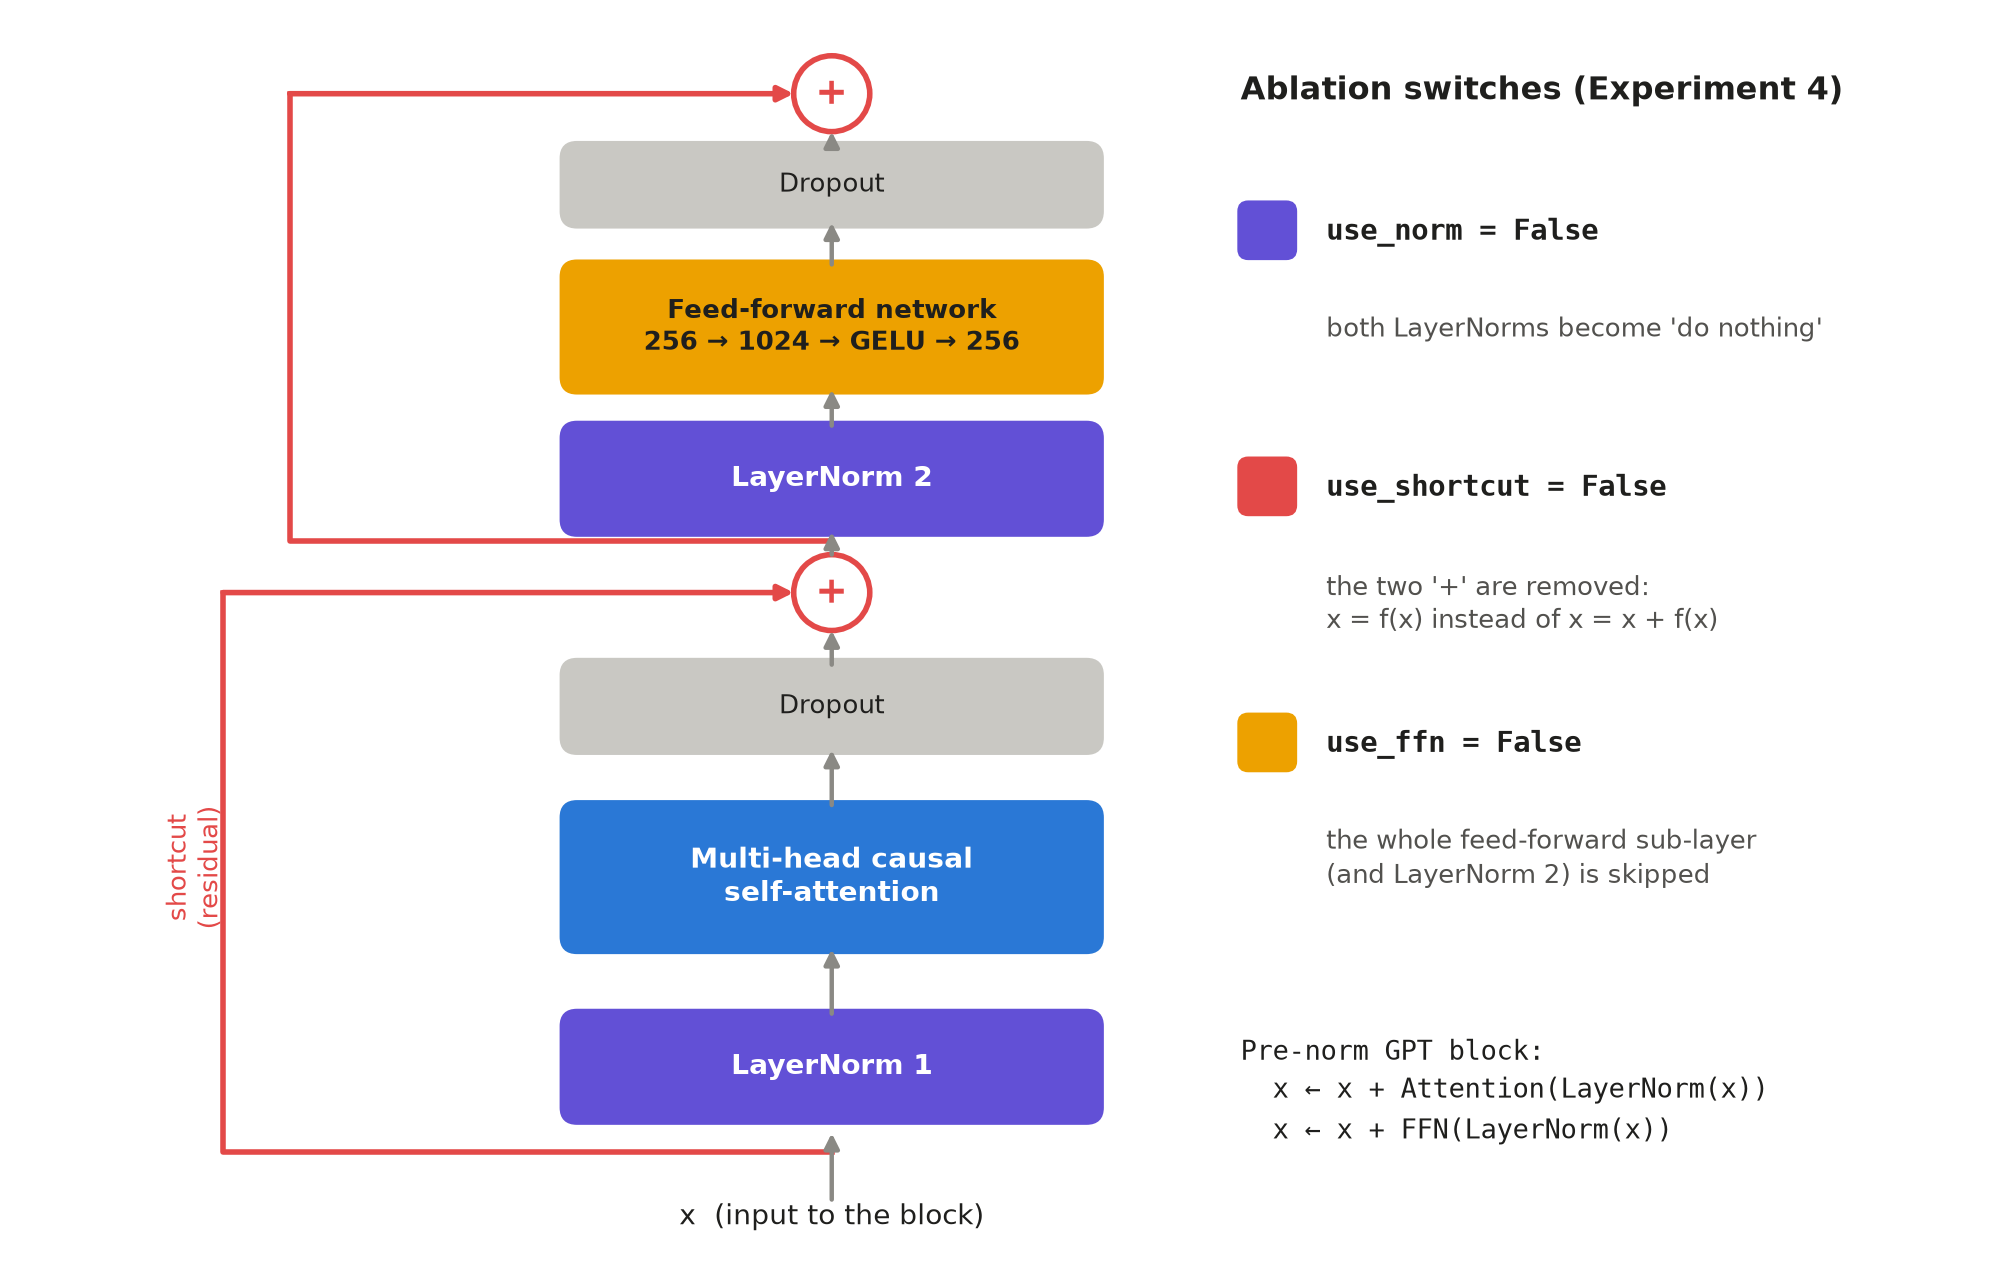
\includegraphics[width=0.82\textwidth]{transformer_block.png}
  \caption{The pre-norm transformer block used in this study and the three ablation switches. Each switch removes the component from \emph{every} block; the final LayerNorm before the output head is always kept.}
  \label{fig:block}
\end{figure}

\subsection{Expected roles of the components}
\begin{itemize}[leftmargin=*]
  \item \textbf{Residual connections} give gradients a direct path to early layers and let each block learn a small correction to its input; without them deep networks suffer from vanishing gradients~\cite{he2016resnet}.
  \item \textbf{LayerNorm} keeps activations at a stable scale, which allows larger learning rates and deeper stacks~\cite{ba2016layernorm}; the pre-norm placement is known to stabilise transformer training~\cite{xiong2020prenorm}.
  \item \textbf{The FFN} holds about two thirds of each block's parameters and has been shown to act as a key-value memory that stores much of a model's knowledge~\cite{geva2021ffn}.
  \item \textbf{Multiple heads} let a layer attend to several patterns at once, although many heads can be pruned in trained models with little loss~\cite{michel2019sixteen}.
  \item \textbf{Scale.} Loss improves predictably with model size and data, and compute-optimal training uses roughly 20 tokens per parameter~\cite{kaplan2020scaling,hoffmann2022chinchilla}. Our setting is far from this: about $0.006$ tokens per parameter.
\end{itemize}

% =====================================================================
\section{Experimental Setup}\label{sec:setup}

\subsection{Data}
The corpus is \emph{Pride and Prejudice} (Project Gutenberg, book 1342). We remove the Gutenberg licence header and footer, the \texttt{[Illustration]} captions and the indentation used for centred titles, and collapse repeated blank lines. The text is tokenised with the GPT-2 byte-pair encoding~\cite{sennrich2016bpe,radford2019gpt2}. The first 90\% of tokens form the training set and the last 10\% the validation set, so validation consists of complete final chapters that never appear in training. Both sets are cut into non-overlapping windows of 256 tokens; the target of each window is the input shifted by one token. \Cref{tab:dataset} summarises the data.

\begin{table}[h]
  \centering
  \caption{Dataset statistics.}
  \label{tab:dataset}
  \begin{tabular}{lr}
\toprule
Quantity & Value \\
\midrule
Characters after cleaning & 718,925 \\
Total tokens (GPT-2 BPE) & 186,785 \\
Training tokens (first 90\%) & 168,106 \\
Validation tokens (last 10\%) & 18,679 \\
Context length & 256 \\
Training / validation sequences & 656 / 72 \\
Batch size / steps per epoch & 16 / 41 \\
\bottomrule
\end{tabular}

\end{table}

\subsection{Model}
The model follows GPT-2~\cite{radford2019gpt2,raschka2024llm} but is scaled down so that the study fits on a free GPU (\cref{tab:model}). With the base configuration it has 28,953,600 parameters. Of these, 25.7M (89\%) belong to the token embedding and the output head ($2 \times 50{,}257 \times 256$); each transformer block has 788,992 parameters, of which 525,568 (66.6\%) are in the FFN and 262,400 in attention. Changing the depth from 1 to 12 layers therefore changes the total only from 26.6M to 35.3M, and removing the FFN saves 2.1M parameters with 4 layers and 6.3M with 12. The number of heads does not change the parameter count.

\begin{table}[h]
  \centering
  \small
  \caption{Base model configuration. Experiments 2--4 change one entry at a time.}
  \label{tab:model}
  \begin{tabular}{lll}
    \toprule
    Setting & Value & Note \\
    \midrule
    Vocabulary size & 50,257 & GPT-2 BPE tokenizer \\
    Context length & 256 & GPT-2: 1,024 \\
    Embedding dimension $d$ & 256 & GPT-2: 768 \\
    Attention heads $H$ & 4 & varied in Experiment 3 \\
    Transformer layers & 4 & varied in Experiment 2 \\
    Dropout~\cite{srivastava2014dropout} & 0.1 & embeddings, attention, residual branches \\
    QKV bias & no & as in GPT-2 \\
    Initialisation & $\mathcal{N}(0, 0.02^2)$, zero biases & GPT-2 scheme \\
    \bottomrule
  \end{tabular}
\end{table}

\subsection{Training and evaluation protocol}
Every run is produced by a single training function, so runs differ only in the factor under study (\cref{tab:protocol}). We use AdamW~\cite{loshchilov2019adamw} with a \emph{constant} learning rate and clip the global gradient norm at 1.0~\cite{pascanu2013difficulty}. After every epoch we measure the training loss on a fixed random subset of 160 training sequences and the validation loss on all 72 validation sequences, both in evaluation mode (dropout off), and we record the mean gradient norm before clipping.

Because every configuration eventually overfits, the final loss depends mainly on how long a model was trained. Our primary metric is therefore the \textbf{best validation loss} and the epoch at which it occurs (the \emph{best epoch}), i.e.\ the result early stopping would select.

\begin{table}[h]
  \centering
  \small
  \caption{Training and evaluation protocol shared by all runs.}
  \label{tab:protocol}
  \begin{tabularx}{\textwidth}{@{}lX@{}}
    \toprule
    Item & Setting \\
    \midrule
    Optimiser & AdamW, $\beta=(0.9, 0.999)$, weight decay 0.1 \\
    Learning-rate schedule & constant (no warm-up, no decay) \\
    Gradient clipping & global norm 1.0 \\
    Batch size & 16 sequences of 256 tokens (41 steps per epoch) \\
    Precision & fp16 mixed precision with gradient scaling \\
    Seed & 123 (Experiments 2--3 additionally 42 and 7) \\
    Evaluation & every epoch: train loss (160 fixed sequences), validation loss (all 72) \\
    Text samples & prompt ``I am sure that'', 50 tokens, temperature 0.8, top-$k$ 40, seed 123 \\
    Hardware & NVIDIA T4 (Google Colab) \\
    \bottomrule
  \end{tabularx}
\end{table}

\subsection{Count-based reference models}\label{sec:reference}
To interpret loss values, we evaluate two models that only count tokens in the training set and need no training:
\begin{itemize}[leftmargin=*]
  \item a \textbf{unigram} model, $p(x_{t+1}) = (c(x_{t+1}) + \alpha)/(N + \alpha|V|)$ with $\alpha=0.1$, which knows only how frequent each token is; and
  \item an interpolated \textbf{bigram} model, $p(x_{t+1}\mid x_t) = \lambda\, c(x_t, x_{t+1})/c(x_t) + (1-\lambda)\,p_{\text{uni}}(x_{t+1})$ with $\lambda = 0.7$, which conditions on the previous token only.
\end{itemize}
On the validation set they reach \textbf{6.32} and \textbf{4.94}. The value of $\lambda$ was chosen on the validation set from $\{0.3,\dots,0.8\}$, so 4.94 is a slightly optimistic reference. \Cref{tab:reference} places these values on one scale together with our main results.

\begin{table}[h]
  \centering
  \caption{Reference points for interpreting the loss (validation set, nats per token).}
  \label{tab:reference}
  \begin{tabular}{lrrl}
    \toprule
    Model & Loss & PPL & What it captures \\
    \midrule
    Uniform guessing & 10.82 & 50,257 & nothing \\
    Unigram counts & 6.32 & 556 & token frequency only \\
    Bigram counts & 4.94 & 140 & previous token only \\
    Best transformer (this work) & 4.61 & 101 & up to 256 tokens of context \\
    \bottomrule
  \end{tabular}
\end{table}

\subsection{Reproducibility and sanity checks}
A fixed seed (123) controls the initial weights, the shuffling of training sequences, dropout masks and text sampling, so repeated runs give the same result up to small non-determinism in GPU kernels. Each finished run is stored as a JSON file named after its full configuration, and is reloaded rather than retrained when the same configuration appears again. Long runs are checkpointed every 25 epochs. Before the experiments we verified that (i) the untrained model's loss is close to $\ln|V| = 10.82$ (observed: 10.859), (ii) the model can drive the loss on a single batch close to zero (0.042 after 200 steps), and (iii) all ablation variants produce finite logits of the expected shape. The full study comprises 47 runs and about 4.2 GPU-hours. The notebook, including all training logs, figures and tables, can be opened and re-run at \href{\colaburl}{this Colab link}.

% =====================================================================
\section{Baseline}\label{sec:baseline}

The baseline uses the base configuration, learning rate $4\times10^{-4}$ and 20 epochs (\cref{fig:baseline}). Training and validation loss fall together for the first few epochs. The best validation loss, \textbf{4.616} (perplexity 101), is reached at \textbf{epoch 10}. After that the training loss keeps falling (to 2.47 at epoch 20) while the validation loss rises to 4.97: the model has started to overfit. Training took 1.4 minutes. This learning rate later turned out to give the lowest validation loss of any full model in the study.

\begin{figure}[h]
  \centering
  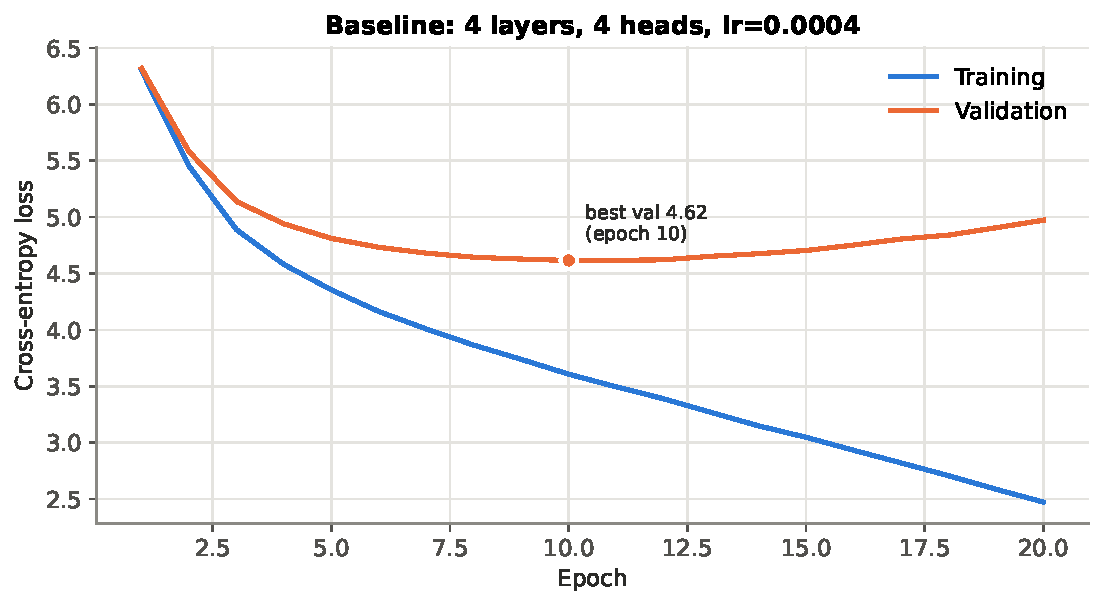
\includegraphics[width=0.72\textwidth]{baseline_loss.pdf}
  \caption{Baseline (4 layers, 4 heads, LR $4\times10^{-4}$). The dot marks the best validation loss.}
  \label{fig:baseline}
\end{figure}

% =====================================================================
\section{Experiment 1: Epochs and Learning Rate}\label{sec:exp1}

\paragraph{Design.} We test learning rates of $10^{-4}$, $10^{-3}$ and $10^{-2}$ and read off the losses after 5, 10, 20, 50, 100, 200 and 500 epochs. Because the learning rate is constant and the seed is fixed, a 500-epoch run passes through every shorter setting exactly as a separate run would. We therefore train one 500-epoch run per learning rate (3 runs instead of 21). A separate 20-epoch run at $10^{-3}$ confirmed this: its validation curve matches the first 20 epochs of the long run to within 0.02. The remaining difference comes from non-deterministic GPU arithmetic accumulating over 20 epochs. It is of the same order as the seed-to-seed variation reported in \cref{sec:exp2,sec:exp3}, which is a further reason to treat differences below about 0.02 as noise.

\begin{figure}[t]
  \centering
  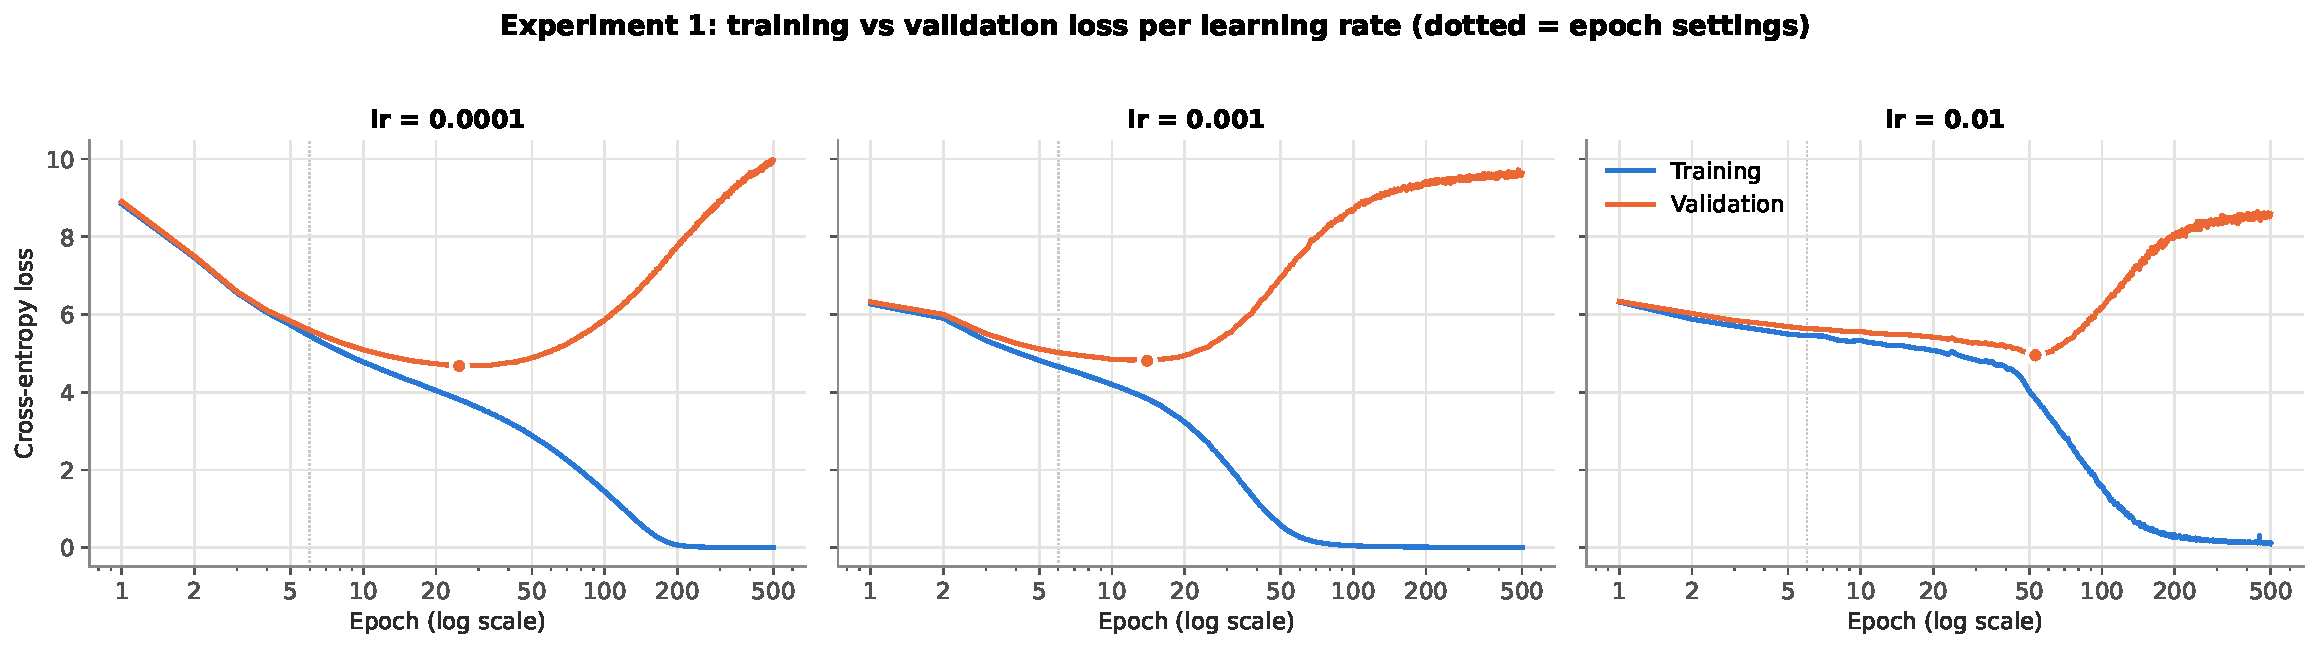
\includegraphics[width=\textwidth]{exp1_per_lr.pdf}
  \caption{Training and validation loss for each learning rate over 500 epochs (logarithmic epoch axis). Dots mark the best validation loss; dotted lines mark the evaluated epoch settings.}
  \label{fig:exp1}
\end{figure}

\begin{table}[t]
  \centering
  \caption{Loss after $N$ epochs for each learning rate. Bold: lowest validation loss among the evaluated epoch settings.}
  \label{tab:exp1grid}
  \begin{tabular}{lrrrrrrr}
\toprule
& \multicolumn{7}{c}{Epochs} \\
\cmidrule(lr){2-8}
LR & 5 & 10 & 20 & 50 & 100 & 200 & 500 \\
\midrule
\multicolumn{8}{l}{\emph{Validation loss}} \\
$1\times10^{-4}$ & 5.83 & 5.09 & \textbf{4.73} & 4.88 & 5.85 & 7.77 & 9.97 \\
$1\times10^{-3}$ & 5.11 & \textbf{4.84} & 4.95 & 6.95 & 8.71 & 9.38 & 9.64 \\
$1\times10^{-2}$ & 5.69 & 5.57 & 5.42 & \textbf{4.99} & 6.17 & 8.00 & 8.59 \\
\midrule
\multicolumn{8}{l}{\emph{Training loss}} \\
$1\times10^{-4}$ & 5.73 & 4.78 & 4.05 & 2.88 & 1.45 & 0.07 & 0.01 \\
$1\times10^{-3}$ & 4.82 & 4.20 & 3.23 & 0.59 & 0.05 & 0.01 & 0.01 \\
$1\times10^{-2}$ & 5.50 & 5.33 & 5.07 & 4.03 & 1.57 & 0.27 & 0.11 \\
\bottomrule
\end{tabular}

\end{table}

\begin{table}[t]
  \centering
  \caption{Experiment 1 summary (500 epochs per learning rate).}
  \label{tab:exp1}
  \begin{tabular}{lrrrrrr}
\toprule
LR & Best val. & Best epoch & PPL & Train @500 & Val. @500 & Minutes \\
\midrule
$1\times10^{-4}$ & 4.676 & 25 & 107.3 & 0.006 & 9.973 & 36.2 \\
$1\times10^{-3}$ & 4.809 & 14 & 122.7 & 0.009 & 9.645 & 35.8 \\
$1\times10^{-2}$ & 4.951 & 53 & 141.4 & 0.113 & 8.588 & 35.7 \\
\bottomrule
\end{tabular}

\end{table}

\paragraph{Results.} \Cref{fig:exp1,tab:exp1grid,tab:exp1} show the same pattern for every learning rate:
\begin{itemize}[leftmargin=*]
  \item \textbf{U-shaped validation loss.} Validation loss falls, reaches a minimum, then rises steadily. The training loss falls monotonically to $0.006$ ($10^{-4}$) and $0.009$ ($10^{-3}$): the model memorises the training chapters.
  \item \textbf{Extreme overfitting with long training.} After 500 epochs the validation loss is 9.97, 9.65 and 8.59, close to uniform guessing (10.82). A memorised model is highly confident, so its errors on unseen text are penalised heavily by the cross-entropy. The generalisation gap grows accordingly (\cref{fig:exp1gap}).
  \item \textbf{A higher learning rate overfits sooner.} The best epoch moves from 25 ($10^{-4}$) to 14 ($10^{-3}$).
  \item \textbf{$10^{-2}$ is noisy but stable.} With AdamW and gradient clipping no run diverged, but at $10^{-2}$ the validation loss improved only slowly (5.69 at epoch 5, 4.99 at epoch 50). Its minimum (4.951 at epoch 53) was followed by a sudden drop in training loss as memorisation began.
  \item \textbf{The smaller learning rate reached the lower minimum} (4.676 vs.\ 4.809 vs.\ 4.951). The baseline rate $4\times10^{-4}$ was better still (4.616), so the optimum lies between $10^{-4}$ and $10^{-3}$ and the tested grid is coarse.
\end{itemize}

\begin{figure}[t]
  \centering
  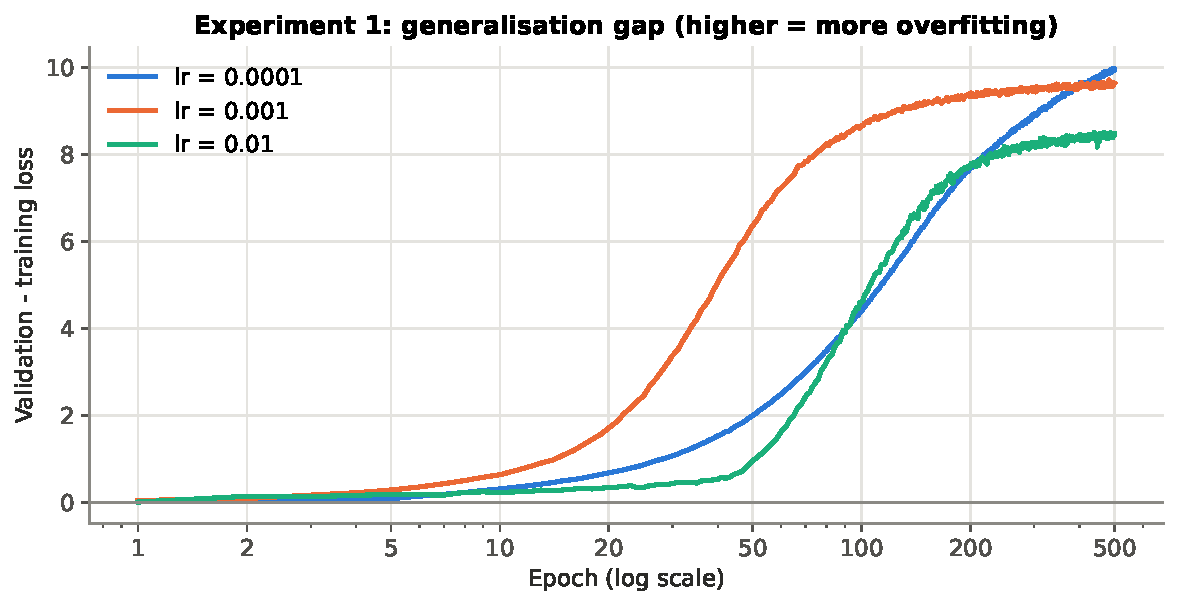
\includegraphics[width=0.66\textwidth]{exp1_gap.pdf}
  \caption{Generalisation gap (validation minus training loss) over training.}
  \label{fig:exp1gap}
\end{figure}

\paragraph{Answer to RQ1.} On this corpus the useful training horizon is short: 10--25 epochs depending on the learning rate. Additional epochs only add memorisation. The learning rate controls both how fast the model learns and how soon it begins to overfit.

\paragraph{Settings for Experiments 2--4.} Architecture experiments require a fixed optimisation setting. The notebook selected the learning rate with the lowest best validation loss in Experiment~1 ($10^{-4}$) and $\lceil 1.5\times \text{its best epoch}\rceil = 38$ epochs, so that the curves also show the onset of overfitting. \Cref{sec:exp4} shows that this low learning rate and fixed budget bias some comparisons; the ablations were therefore repeated under a revised protocol.

% =====================================================================
\section{Experiment 2: Number of Transformer Layers}\label{sec:exp2}

We train models with 1, 3, 5, 7 and 12 layers (4 heads, LR $10^{-4}$, 38 epochs). Because the differences in the first run were small, every depth was repeated with seeds 42 and 7.

\begin{figure}[t]
  \centering
  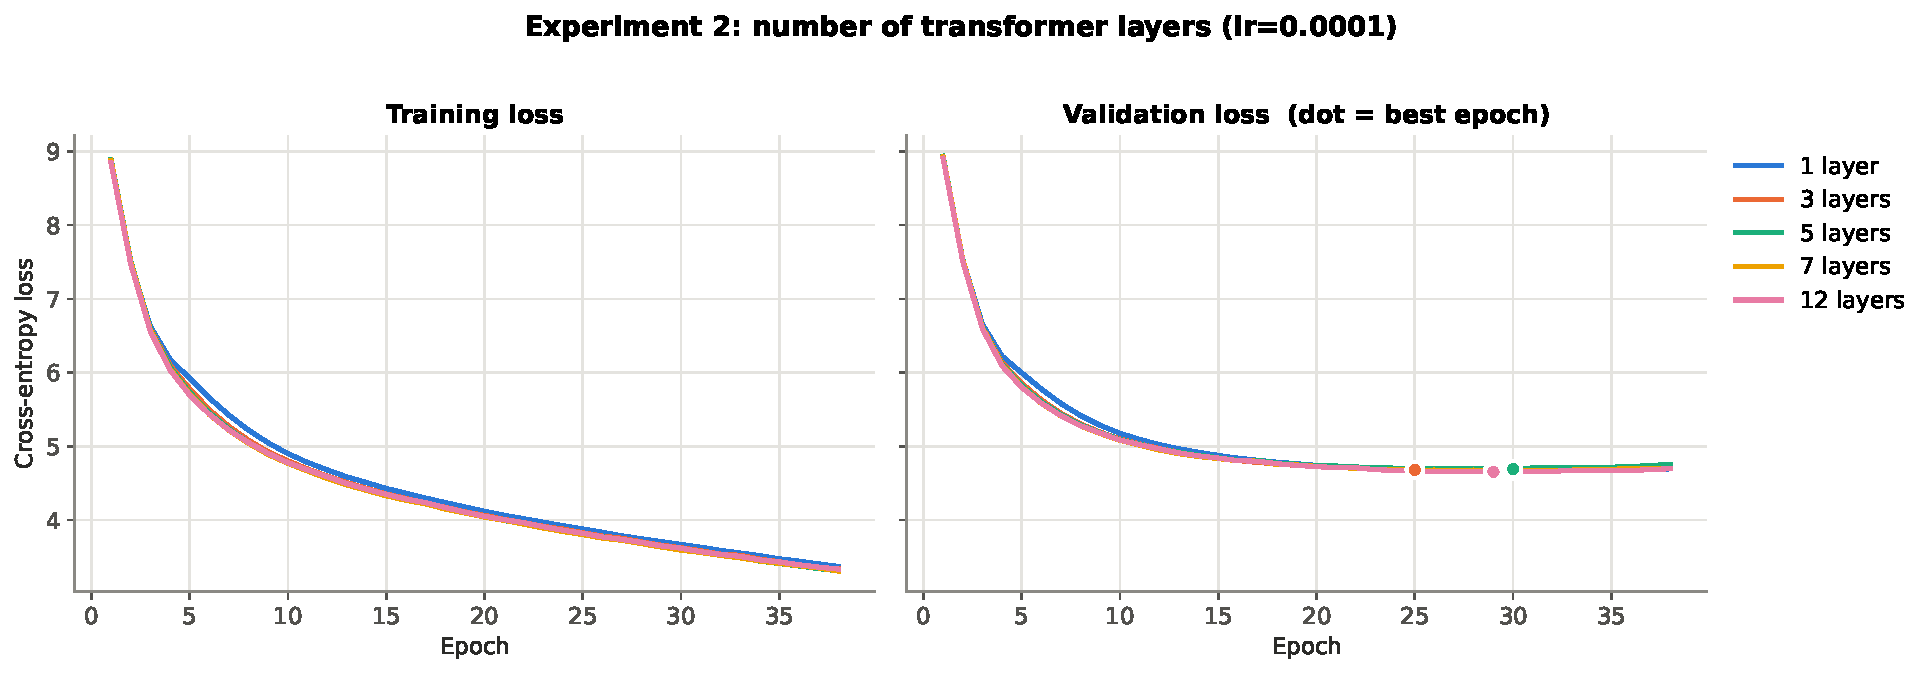
\includegraphics[width=\textwidth]{exp2_layers.pdf}
  \caption{Training and validation loss for different depths (seed 123). The curves almost coincide.}
  \label{fig:exp2}
\end{figure}

\begin{figure}[t]
  \centering
  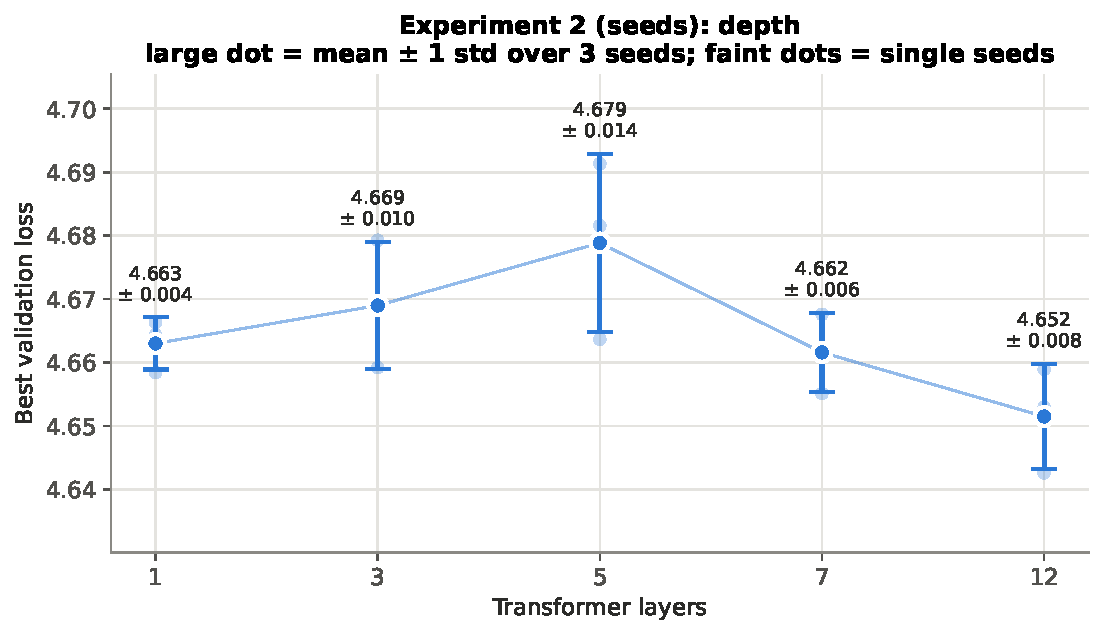
\includegraphics[width=0.66\textwidth]{exp2_seeds.pdf}
  \caption{Best validation loss against depth over three seeds (mean $\pm$ one standard deviation; faint dots are individual seeds).}
  \label{fig:exp2seeds}
\end{figure}

\begin{table}[t]
  \centering
  \caption{Experiment 2: depth. PPL is the perplexity of the three-seed mean.}
  \label{tab:exp2}
  \begin{tabular}{rrrrcrr}
\toprule
& & \multicolumn{2}{c}{Seed 123} & \multicolumn{2}{c}{3 seeds (123, 42, 7)} & \\
\cmidrule(lr){3-4}\cmidrule(lr){5-6}
Layers & Params (M) & Best val. & Epoch & Mean $\pm$ std & PPL & Min./run \\
\midrule
1 & 26.59 & 4.664 & 30 & $4.663 \pm 0.004$ & 106.0 & 2.4 \\
3 & 28.16 & 4.679 & 25 & $4.669 \pm 0.010$ & 106.6 & 2.6 \\
5 & 29.74 & 4.691 & 30 & $4.679 \pm 0.014$ & 107.7 & 2.8 \\
7 & 31.32 & 4.668 & 29 & $4.662 \pm 0.006$ & 105.8 & 3.0 \\
12 & 35.27 & 4.653 & 29 & $4.652 \pm 0.008$ & 104.7 & 3.5 \\
\bottomrule
\end{tabular}

\end{table}

\paragraph{Results.} The training and validation curves for all depths are nearly identical (\cref{fig:exp2}); even the training loss after 38 epochs differs by only 0.06 (3.31--3.37). Over three seeds (\cref{fig:exp2seeds,tab:exp2}) the best validation loss ranges from $4.652$ (12 layers) to $4.679$ (5 layers) without a monotonic trend: it rises from 1 to 5 layers and falls again at 7 and 12. The seed-to-seed standard deviation is 0.004--0.014. The difference between the best and worst depth (0.027) is about three times the average standard deviation, but most error bars overlap and only 12 versus 5 layers separate clearly. Meanwhile, the time per epoch grows by about 45\% from 1 to 12 layers.

\paragraph{Answer to RQ2.} On this dataset depth has no consistent effect. Extra layers add capacity, but the models memorise the corpus before that capacity can improve generalisation (\cref{sec:discussion}).

% =====================================================================
\section{Experiment 3: Number of Attention Heads}\label{sec:exp3}

We train models with 1, 2, 4 and 8 heads at a fixed width of 256, so the head dimension is 256, 128, 64 and 32. The parameter count is identical for all four models, so this experiment changes only how attention capacity is divided.

\begin{figure}[t]
  \centering
  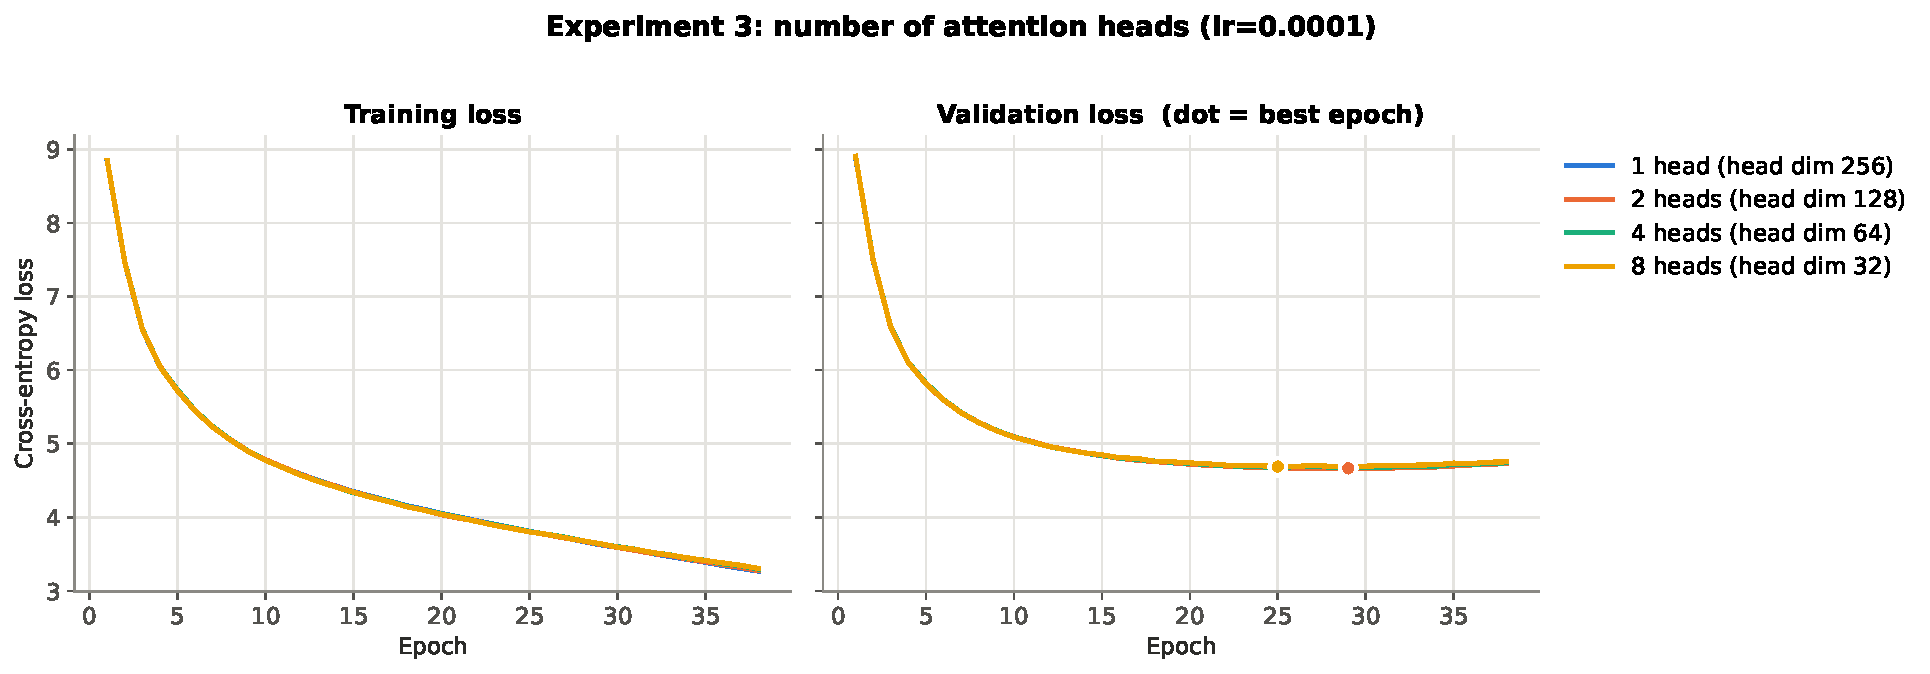
\includegraphics[width=\textwidth]{exp3_heads.pdf}
  \caption{Training and validation loss for different numbers of heads (seed 123).}
  \label{fig:exp3}
\end{figure}

\begin{figure}[t]
  \centering
  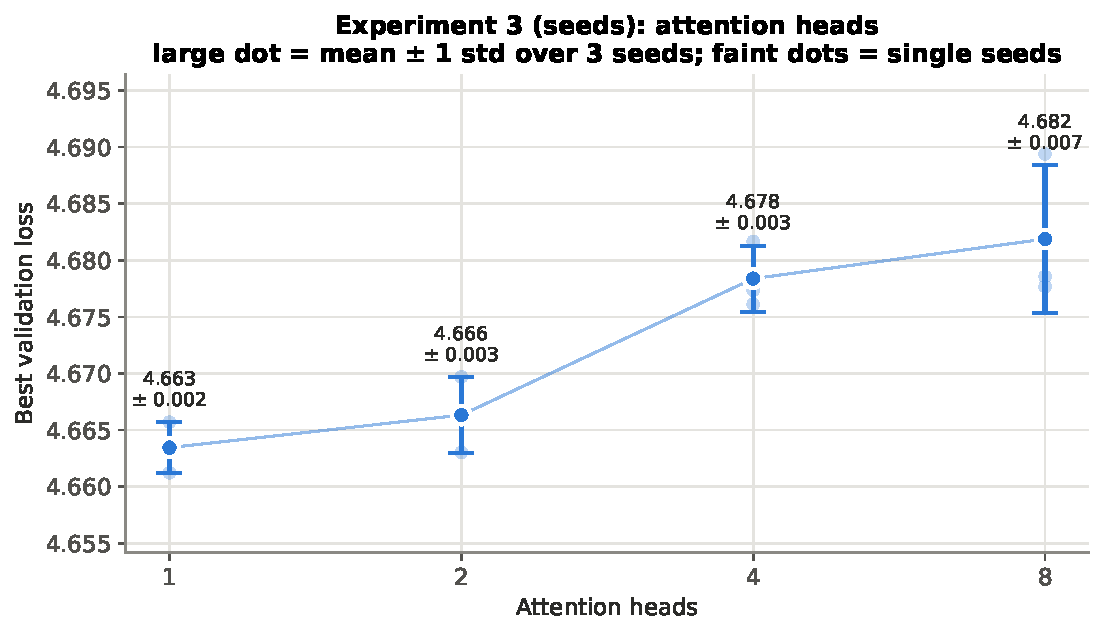
\includegraphics[width=0.66\textwidth]{exp3_seeds.pdf}
  \caption{Best validation loss against the number of heads over three seeds.}
  \label{fig:exp3seeds}
\end{figure}

\begin{table}[t]
  \centering
  \caption{Experiment 3: attention heads at fixed width $d=256$.}
  \label{tab:exp3}
  \begin{tabular}{rrrrcr}
\toprule
& & \multicolumn{2}{c}{Seed 123} & \multicolumn{2}{c}{3 seeds (123, 42, 7)} \\
\cmidrule(lr){3-4}\cmidrule(lr){5-6}
Heads & Head dim. & Best val. & Epoch & Mean $\pm$ std & PPL \\
\midrule
1 & 256 & 4.666 & 29 & $4.663 \pm 0.002$ & 106.0 \\
2 & 128 & 4.666 & 29 & $4.666 \pm 0.003$ & 106.3 \\
4 & 64 & 4.676 & 25 & $4.678 \pm 0.003$ & 107.6 \\
8 & 32 & 4.689 & 25 & $4.682 \pm 0.006$ & 108.0 \\
\bottomrule
\end{tabular}

\end{table}

\paragraph{Results.} The best validation loss increases monotonically with the number of heads: $4.663$ (1 head), $4.666$ (2), $4.678$ (4) and $4.682$ (8) (\cref{fig:exp3seeds,tab:exp3}). The seed-to-seed standard deviation is very small (0.002--0.007), and the 1-versus-8 difference (0.018) is about five times the average standard deviation, so the ordering is reliable. The effect itself is small, about 2\% in perplexity (106 vs.\ 108).

\paragraph{Answer to RQ3.} With the width fixed, fewer and wider heads are slightly better here. Splitting 256 dimensions into eight 32-dimensional heads makes each query-key comparison lower-dimensional, while a single book appears to require only a few distinct attention patterns. This differs from the usual large-scale setting, where many heads are standard, and is consistent with observations that many heads are redundant~\cite{michel2019sixteen}.

% =====================================================================
\section{Experiment 4: Ablation Studies}\label{sec:exp4}

Each ablation removes one component from every transformer block (\cref{fig:block}): both LayerNorms (\texttt{use\_norm=False}), both residual additions (\texttt{use\_shortcut=False}, so $y=f(x)$), or the FFN sub-layer (\texttt{use\_ffn=False}). Ablations are run with 4 layers and, because residual connections and normalisation are expected to matter more in deep networks, also with 12 layers.

\subsection{Initial protocol: LR \texorpdfstring{$10^{-4}$}{1e-4}, 38 epochs}

\begin{figure}[t]
  \centering
  \begin{subfigure}{\textwidth}
    \centering
    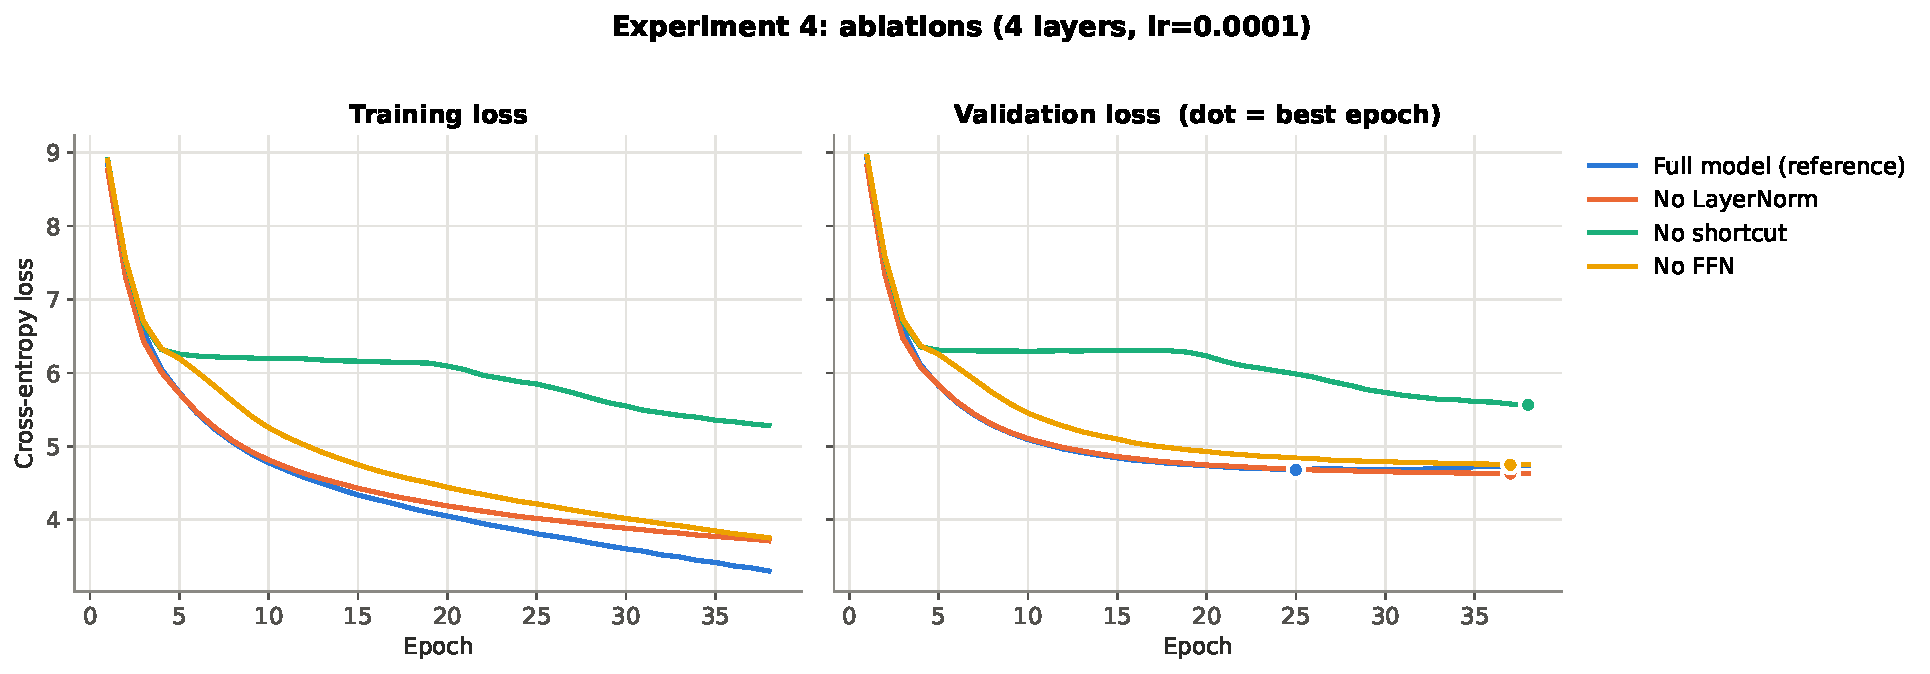
\includegraphics[width=\textwidth]{exp4_ablations.pdf}
    \caption{4 layers}
  \end{subfigure}\\[4pt]
  \begin{subfigure}{\textwidth}
    \centering
    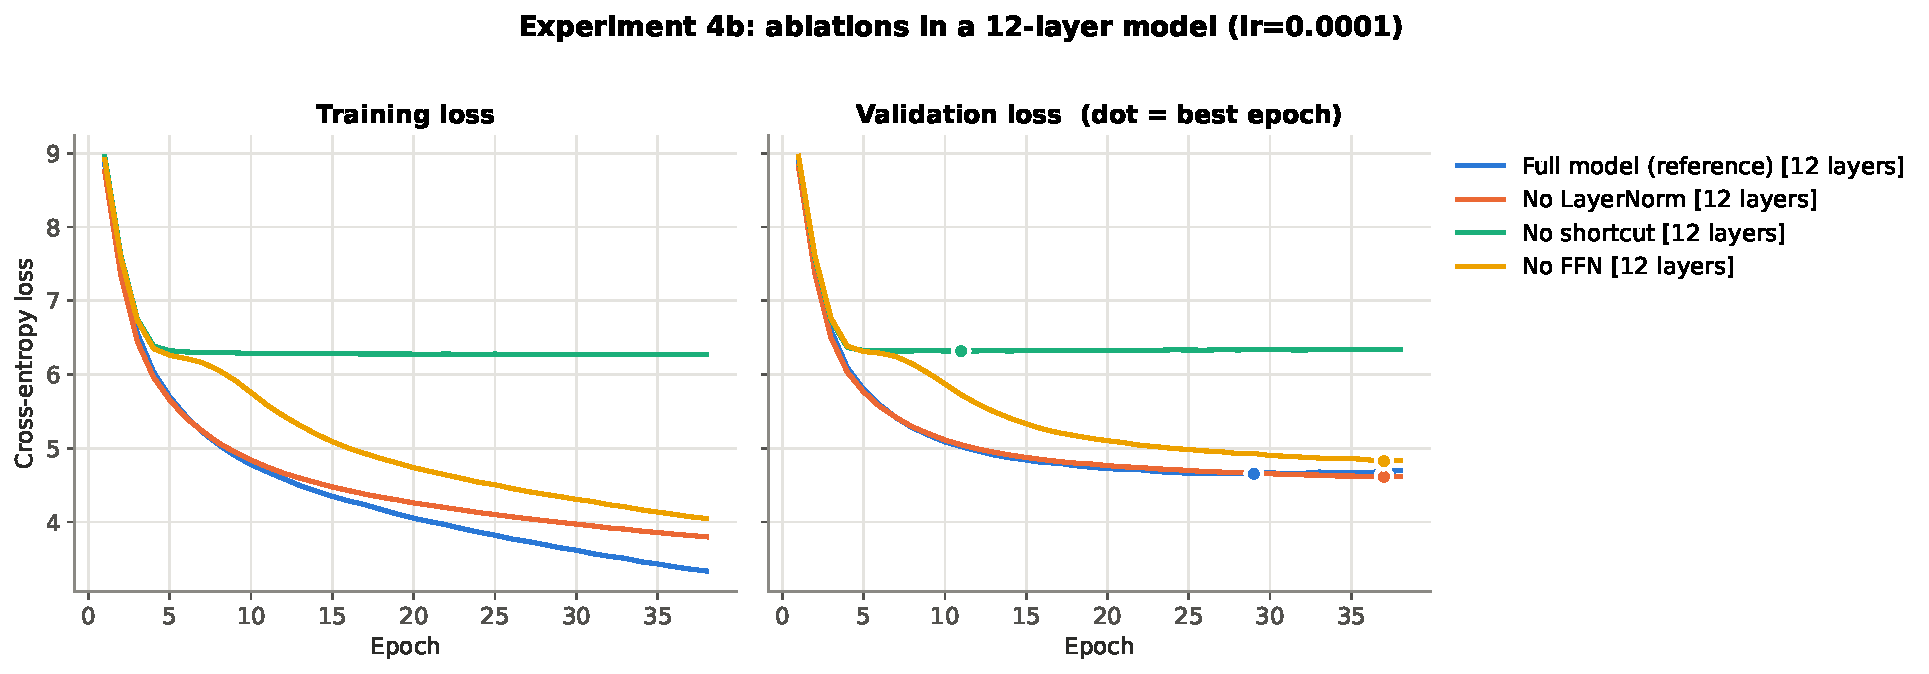
\includegraphics[width=\textwidth]{exp4b_deep_ablations.pdf}
    \caption{12 layers}
  \end{subfigure}
  \caption{Ablations under the initial protocol (LR $10^{-4}$, 38 epochs).}
  \label{fig:exp4}
\end{figure}

\begin{table}[t]
  \centering
  \caption{Ablations under the initial protocol (LR $10^{-4}$, 38 epochs). Upper block: 4 layers; lower block: 12 layers.}
  \label{tab:exp4initial}
  \small
  \begin{tabular}{lrrrrrr}
\toprule
Variant & Layers & Params (M) & Best val. & Best epoch & Final train & Final val. \\
\midrule
Full model (reference) & 4 & 28.95 & 4.676 & 25 & 3.299 & 4.741 \\
No LayerNorm & 4 & 28.95 & 4.627 & 37 & 3.710 & 4.630 \\
No shortcut & 4 & 28.95 & 5.564 & 38 & 5.281 & 5.564 \\
No FFN & 4 & 26.85 & 4.747 & 37 & 3.751 & 4.748 \\
\midrule
Full model (reference) & 12 & 35.27 & 4.653 & 29 & 3.335 & 4.696 \\
No LayerNorm & 12 & 35.25 & 4.613 & 37 & 3.799 & 4.616 \\
No shortcut & 12 & 35.27 & 6.316 & 11 & 6.274 & 6.342 \\
No FFN & 12 & 28.95 & 4.824 & 37 & 4.047 & 4.831 \\
\bottomrule
\end{tabular}

\end{table}

Under the setting chosen in Experiment~1 (\cref{fig:exp4,tab:exp4initial}), removing the shortcut clearly hurts (5.564 with 4 layers, 6.316 with 12), removing the FFN appears to hurt (4.747 vs.\ 4.676; 4.824 vs.\ 4.653), and removing LayerNorm appears to help slightly (4.627; 4.613). The \emph{best epoch} column, however, reveals a problem. The full model peaks at epochs 25--29 and then overfits, whereas the variants without LayerNorm or without the FFN peak at epoch 37 of 38: they were still improving when training stopped. The comparison therefore mixes a model past its optimum with models that have not reached theirs. In addition, the low learning rate makes optimisation easy, which may hide the stabilising role of LayerNorm. We therefore repeated the ablations under a revised protocol.

\subsection{Revised protocol: LR \texorpdfstring{$10^{-3}$}{1e-3}, 60 epochs}

All four variants were retrained with 4 and 12 layers at a ten times higher learning rate ($10^{-3}$) and for 60 epochs. Every run reached its minimum by epoch 20 at the latest, well before the end of training, so each model is now compared at its own best epoch (\cref{tab:exp4c}).

\begin{figure}[t]
  \centering
  \begin{subfigure}{\textwidth}
    \centering
    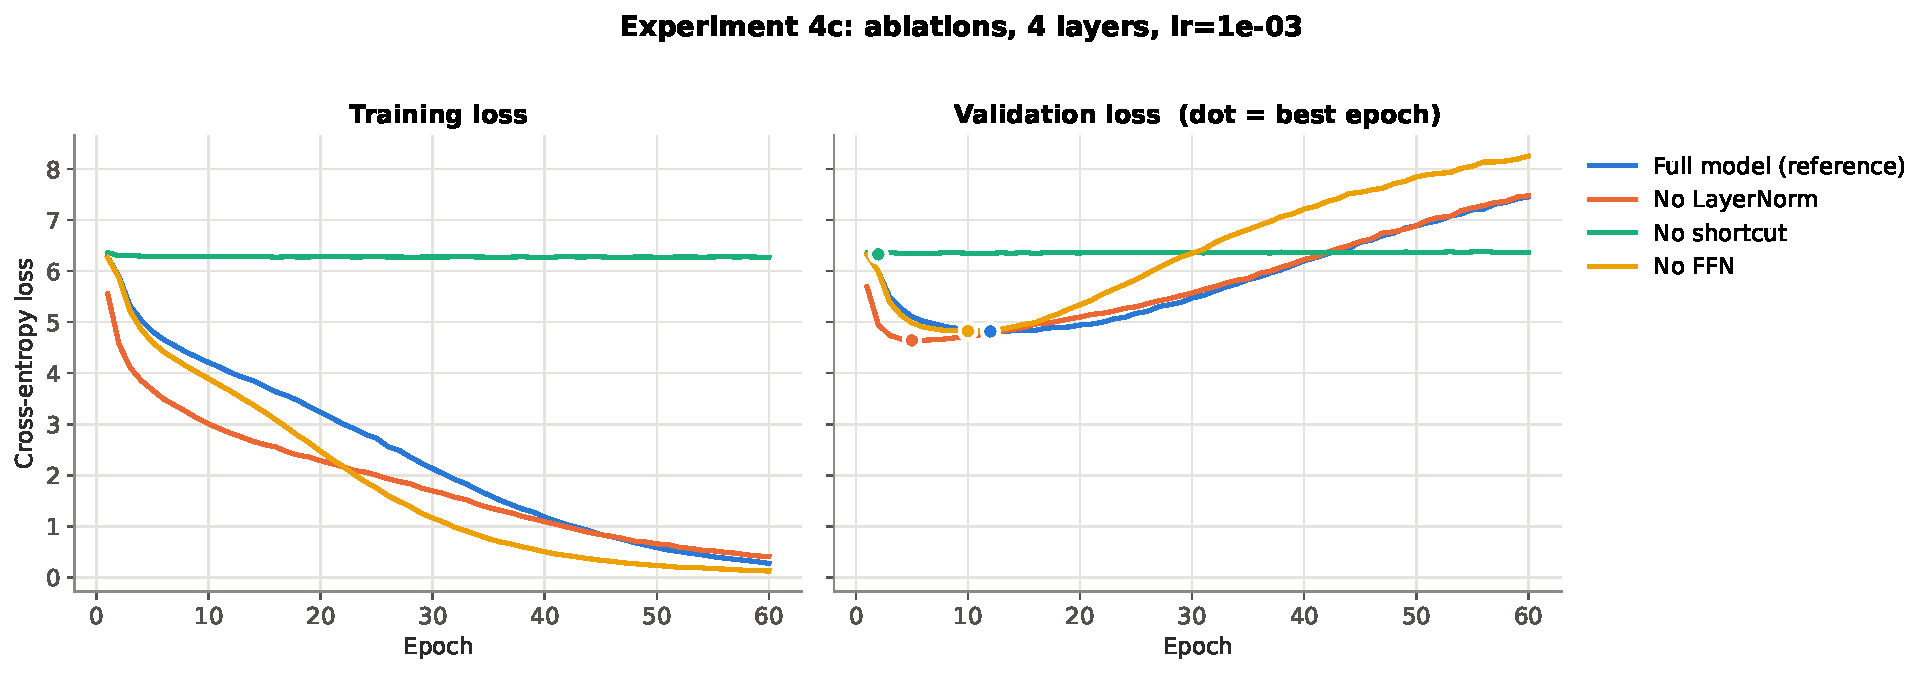
\includegraphics[width=\textwidth]{exp4c_L4_lr0.001_ablations.pdf}
    \caption{4 layers}
  \end{subfigure}\\[4pt]
  \begin{subfigure}{\textwidth}
    \centering
    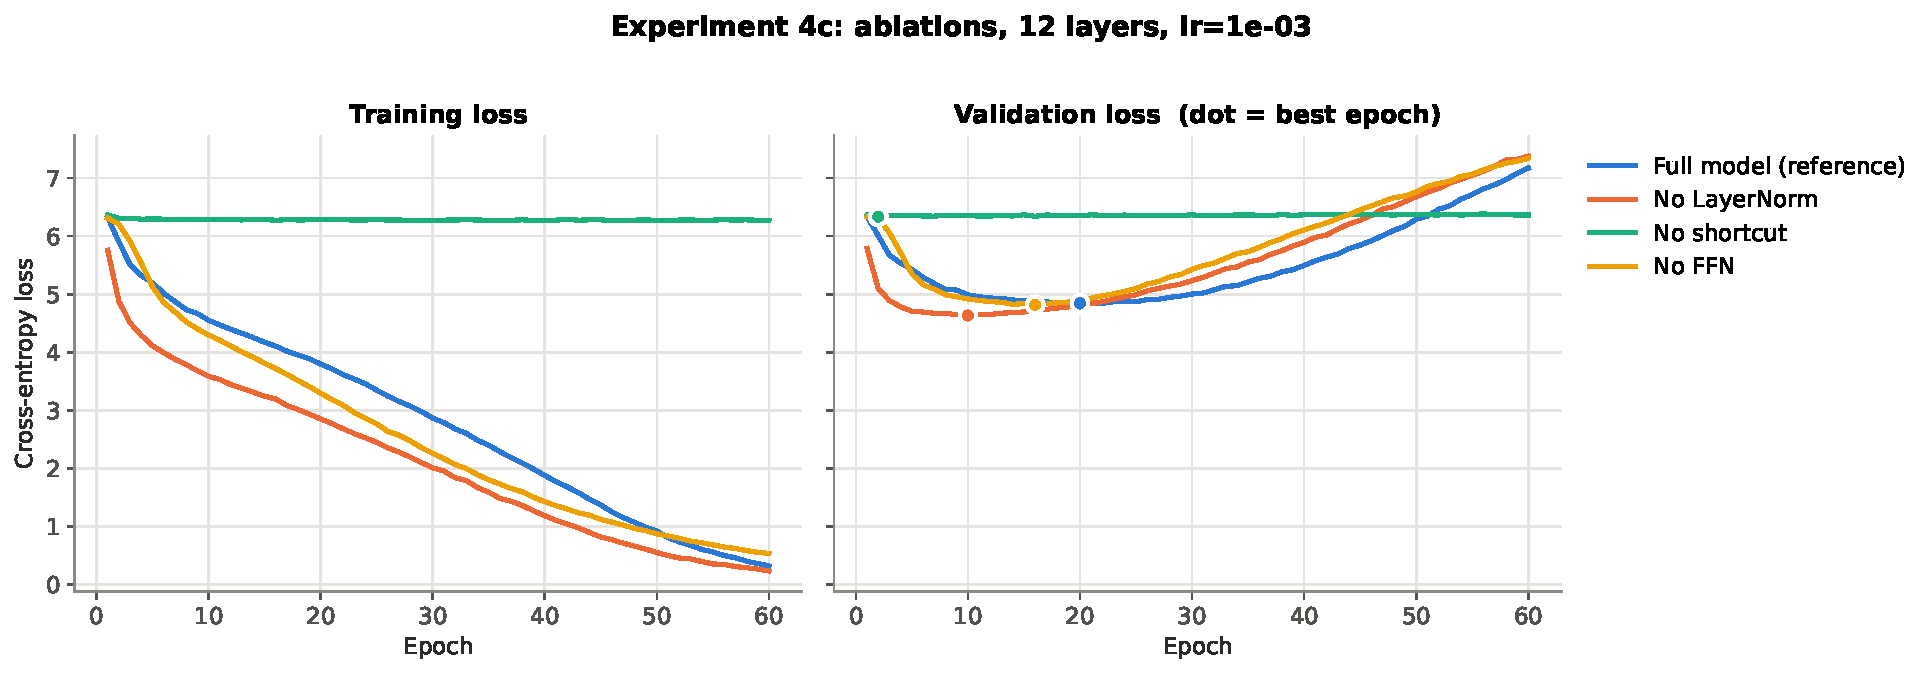
\includegraphics[width=\textwidth]{exp4c_L12_lr0.001_ablations.pdf}
    \caption{12 layers}
  \end{subfigure}
  \caption{Ablations under the revised protocol (LR $10^{-3}$, 60 epochs). Without residual connections (green) the loss stays at the unigram level of about 6.3.}
  \label{fig:exp4c}
\end{figure}

\begin{figure}[t]
  \centering
  \begin{subfigure}{0.49\textwidth}
    \centering
    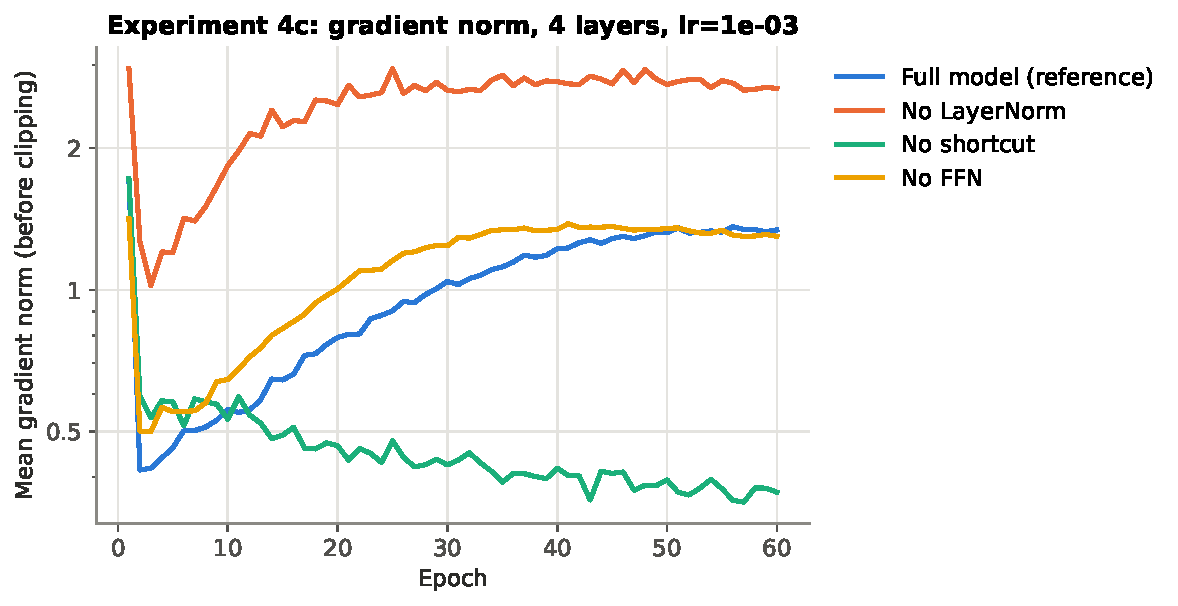
\includegraphics[width=\textwidth]{exp4c_L4_lr0.001_grad_norm.pdf}
    \caption{4 layers}
  \end{subfigure}\hfill
  \begin{subfigure}{0.49\textwidth}
    \centering
    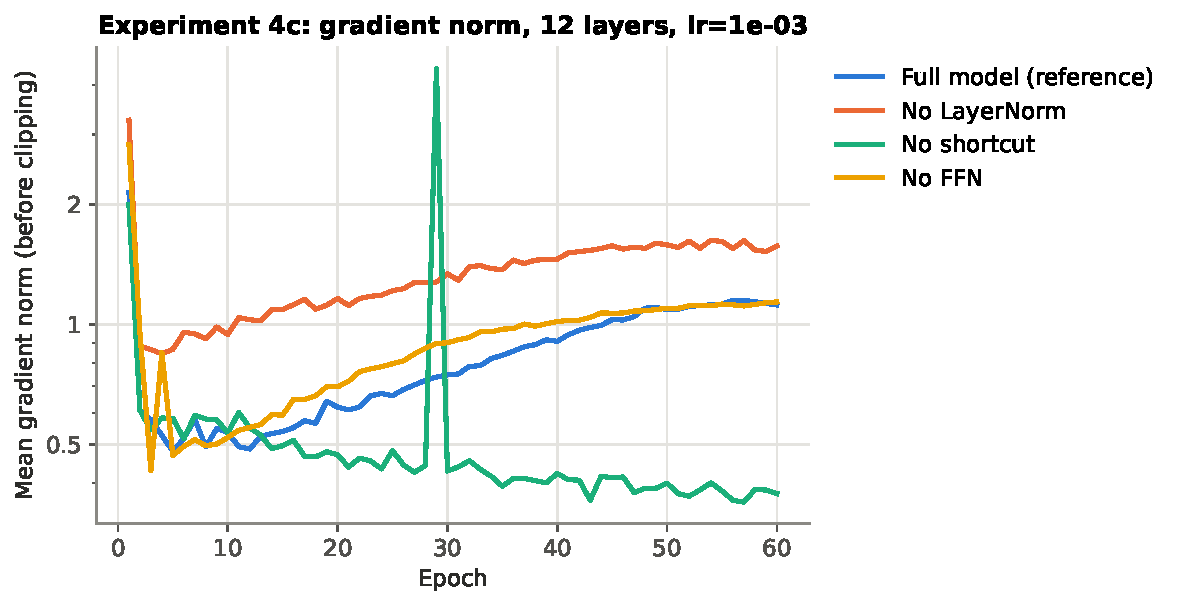
\includegraphics[width=\textwidth]{exp4c_L12_lr0.001_grad_norm.pdf}
    \caption{12 layers}
  \end{subfigure}
  \caption{Mean gradient norm per epoch before clipping (revised protocol, logarithmic axis). Values above 1.0 are clipped to 1.0 before each update.}
  \label{fig:gradnorm}
\end{figure}

\begin{table}[t]
  \centering
  \caption{Best validation loss and best epoch under both protocols, plus the final losses of the revised protocol.}
  \label{tab:exp4c}
  \small
  \begin{tabular}{rlrrrrrr}
\toprule
& & \multicolumn{2}{c}{LR $10^{-4}$, 38 epochs} & \multicolumn{4}{c}{LR $10^{-3}$, 60 epochs} \\
\cmidrule(lr){3-4}\cmidrule(lr){5-8}
L & Variant & Best val. & Epoch & Best val. & Epoch & Final train & Final val. \\
\midrule
4 & Full model (reference) & 4.676 & 25/38 & 4.818 & 12/60 & 0.273 & 7.454 \\
4 & No LayerNorm & 4.627 & 37/38 & 4.642 & 5/60 & 0.403 & 7.476 \\
4 & No shortcut & 5.564 & 38/38 & 6.329 & 2/60 & 6.269 & 6.364 \\
4 & No FFN & 4.747 & 37/38 & 4.823 & 10/60 & 0.123 & 8.250 \\
\midrule
12 & Full model (reference) & 4.653 & 29/38 & 4.841 & 20/60 & 0.320 & 7.171 \\
12 & No LayerNorm & 4.613 & 37/38 & 4.633 & 10/60 & 0.233 & 7.375 \\
12 & No shortcut & 6.316 & 11/38 & 6.333 & 2/60 & 6.269 & 6.363 \\
12 & No FFN & 4.824 & 37/38 & 4.816 & 16/60 & 0.536 & 7.340 \\
\bottomrule
\end{tabular}

\end{table}

\paragraph{Without residual connections the model learns only token frequencies.} At $10^{-3}$ both the 4- and the 12-layer model reach their best validation loss at epoch 2 (6.329 and 6.333) and stay there for the remaining 58 epochs; the training loss also stays at 6.27 (\cref{fig:exp4c}). This value matches the unigram model of \cref{sec:reference} (6.32): the network learns the frequency of each token and nothing about context. Its gradient norm decreases from about 0.6 to 0.3 over training (\cref{fig:gradnorm}), the signature of vanishing gradients when each layer must transform its input completely rather than add a correction. At $10^{-4}$ the 4-layer variant slowly escaped this plateau (5.564); at $10^{-3}$ neither depth did.

\paragraph{Removing LayerNorm improves the best validation loss.} The variant without LayerNorm is better than the full model at both depths and both learning rates: 4.642 vs.\ 4.818 (4 layers) and 4.633 vs.\ 4.841 (12 layers) at $10^{-3}$. Every run converged, and the gap of 0.18--0.21 is about twenty times the seed-to-seed standard deviation measured in Experiments~2--3, so this is not an artefact of the stopping point. Three observations explain it:
\begin{enumerate}[leftmargin=*]
  \item \emph{Gradient clipping substitutes for normalisation.} Without LayerNorm the gradient norm is higher: about 2.4 versus at most 1.2 for the full model with 4 layers, and 0.9--1.6 versus 0.5--1.15 with 12 layers (\cref{fig:gradnorm}). This is the instability that LayerNorm normally prevents, but clipping at 1.0 bounds every update, so training never diverged.
  \item \emph{Faster early learning and an earlier optimum.} Without LayerNorm the validation loss after the first epoch is already about 5.7, versus 6.3 for the full model, and the minimum is reached at epoch 5 instead of 12 (4 layers). One plausible explanation, which we did not test directly, involves the initialisation: with $\mathcal{N}(0,0.02^2)$ weights and no normalisation, the block outputs are initially small, so the network first behaves like a shallow model close to a bigram predictor, which generalises comparatively well on little data. With pre-norm, each block receives unit-scale inputs from the first step and its full capacity becomes available immediately.
  \item \emph{Normalisation is not removed entirely.} The final LayerNorm before the output head is retained, which keeps the logits well scaled.
\end{enumerate}

\paragraph{Removing the FFN has no measurable effect.} Once both models are compared at their best epoch, the variant without FFN equals the full model: 4.823 vs.\ 4.818 (4 layers) and 4.816 vs.\ 4.841 (12 layers), differences within seed variation. The apparent advantage of the FFN under the initial protocol (+0.07 and +0.17) was an artefact of stopping the slower-learning variant before its minimum. After its minimum, the model without FFN overfits most strongly of all variants with 4 layers (final validation loss 8.25).

\paragraph{The higher learning rate itself.} The full model is worse at $10^{-3}$ than at $10^{-4}$ (4.818 vs.\ 4.676 with 4 layers; 4.841 vs.\ 4.653 with 12), in line with Experiment~1: faster optimisation leads to earlier and stronger memorisation of the small corpus. After 60 epochs every variant except the one without shortcuts has a training loss below 0.6 and a validation loss above 7.

\subsection{Inference quality}

\Cref{tab:samples} shows text generated from the same prompt and sampling seed. Early in training the model produces frequent tokens and punctuation; by epoch 10 it produces grammatical fragments with characters and dialogue from the novel. Heavily trained models (epoch 60 at $10^{-3}$, epoch 500) write fluent, Austen-like sentences that are partly recombined from memorised passages. The model without residual connections produces only high-frequency tokens (``as as the,,.''), which matches its unigram-level loss. The variants without LayerNorm and without FFN produce text of similar quality to the full model, consistent with their losses.

\begin{table}[t]
  \centering
  \small
  \caption{Generated continuations of the prompt ``I am sure that''. Samples at epoch 60 come from the end of the revised protocol, not from the best epoch. $\diamond$ marks a partial byte token (half of a curly quotation mark) that cannot be displayed.}
  \label{tab:samples}
  \begin{tabularx}{\textwidth}{@{}p{3.6cm}X@{}}
\toprule
Model & Generated continuation (temperature 0.8, top-$k$ 40, seed 123) \\
\midrule
Baseline, epoch 1 & \emph{I am sure that} as as the,, very that. have. very ; I you $\diamond$,, ,I you was she. you, were,. that $\diamond$ \\ \addlinespace[2pt]
Baseline, epoch 10 & \emph{I am sure that} and the other, for you have a great deal of you himself. I have had not you she\_ did not so certain of my father to \ldots \\ \addlinespace[2pt]
Baseline, epoch 20 & \emph{I am sure that} is not in the being so much disposed of not so much engaged. This I did not likely to be for the next morning at least \ldots \\ \addlinespace[2pt]
LR $10^{-3}$, epoch 500 & \emph{I am sure that} is but the only joined me with you. I had have you have done with an particulars.” “I had my dear Miss Bingley; but I had \ldots \\ \addlinespace[2pt]
Full model, 4L, ep.\ 60 & \emph{I am sure that} when we were very attentive to the very subject.” “If he.” “If he cried Mrs. JenkinsI am sorry with two or little my instrument,” said Mrs. \ldots \\ \addlinespace[2pt]
No LayerNorm, 4L, ep.\ 60 & \emph{I am sure that} theOh, my word is disposed to take it.” Their first thought it of all; but he first witnessing his altered by Derbyshire. And yet seen such \ldots \\ \addlinespace[2pt]
No shortcut, 4L, ep.\ 60 & \emph{I am sure that} as as the,,. be the that., of have. . ; I you ,$\diamond$,, , you was she. you was.,. it that is the \\ \addlinespace[2pt]
No FFN, 4L, ep.\ 60 & \emph{I am sure that} the become of her, and her, and her poultry. or affair is perfectly sure, and Jane may be attended to her, if he had never joined \ldots \\ \addlinespace[2pt]
\bottomrule
\end{tabularx}

\end{table}

\subsection{Answer to RQ4: the role of each component}

\begin{itemize}[leftmargin=*]
  \item \textbf{Residual connections} are what make the network trainable. Without them, even a 4-layer model cannot learn more than token frequencies.
  \item \textbf{LayerNorm} provides stability, but at this depth, with gradient clipping and learning rates up to $10^{-3}$, that stability is not needed; removing it gave better generalisation.
  \item \textbf{The FFN} adds capacity. With one book there is too little to store, so its parameters did not improve validation loss.
\end{itemize}

% =====================================================================
\section{Discussion}\label{sec:discussion}

\paragraph{A data-limited regime.} The model has about 172 parameters per training token, whereas compute-optimal training uses about 20 tokens per parameter~\cite{hoffmann2022chinchilla}. Three observations show that data, not architecture, limits performance here. First, every model memorises the corpus: training loss approaches zero while validation loss rises. Second, all working architectures reach best validation losses in a narrow band (4.61--4.69 under the low learning rate). Third, the best transformer improves on a bigram counting model by only 0.33 nats (4.61 vs.\ 4.94), so most of what the model can extract from 168k tokens is local token statistics. We did not vary the dataset size, so this conclusion is an inference from these observations rather than a direct measurement; it is, however, consistent with scaling-law results~\cite{kaplan2020scaling,hoffmann2022chinchilla}.

\paragraph{Capacity versus trainability.} The ablations separate two kinds of components. \emph{Capacity} components (depth, the FFN, more heads) increase what the model can represent; with little data they mostly accelerate memorisation, and none of them improved validation loss. \emph{Trainability} components (residual connections, LayerNorm) determine whether optimisation succeeds at all. Their importance depends on depth and optimisation settings, not on data size: residual connections were indispensable even for 4 layers, while LayerNorm was unnecessary because the networks were shallow and gradient clipping bounded the updates. We expect LayerNorm to become necessary for deeper networks, higher learning rates or training without clipping, and capacity components to become useful with substantially more data.

\paragraph{Methodological lesson.} The initial protocol, which compared models after a fixed number of epochs with a single seed, led to two conclusions that did not hold up: that the FFN helps, and (as a suspicion) that the LayerNorm result was an artefact. Comparing every model at its own best epoch removed the first, and confirmed the second as a real effect; repeating Experiments~2--3 over three seeds showed that the head effect is real while the depth differences are mostly noise. In a regime where every model overfits, the stopping point and the seed are confounders that must be controlled before architectural conclusions are drawn.

% =====================================================================
\section{Limitations and Future Work}\label{sec:limitations}

\begin{itemize}[leftmargin=*]
  \item \textbf{Single small corpus.} All results come from one novel (168k training tokens). The central claim about data limitation should be tested directly by training on several books (e.g.\ one versus five Austen novels) and checking whether depth and the FFN begin to help.
  \item \textbf{Scaled-down model.} Width 256 and context 256 instead of GPT-2's 768 and 1,024.
  \item \textbf{Simplified optimisation.} A constant learning rate without warm-up or decay, and gradient clipping in every run. Repeating the LayerNorm ablation without clipping and at larger depth would isolate the stabilising role of normalisation.
  \item \textbf{Seeds.} Experiments~2--3 use three seeds, Experiments~1 and~4 one seed. The large ablation effects (shortcut, LayerNorm) are far above the measured seed variation, but the FFN result is within it.
  \item \textbf{Partial normalisation ablation.} The final LayerNorm was kept in the no-LayerNorm variant.
  \item \textbf{Untested mechanism.} The explanation of the faster early learning without LayerNorm is a hypothesis; measuring the scale of each block's output during training would test it.
  \item \textbf{Text samples.} The samples of the revised protocol were taken at the end of training, not at the best epoch.
\end{itemize}

% =====================================================================
\section{Conclusion}\label{sec:conclusion}

We trained a GPT-style model from scratch on one novel and varied training duration, learning rate, depth, attention heads and block components under a controlled protocol. The dominant effect is overfitting: every model reaches its best validation loss within 10--30 epochs and then memorises the training text, and a higher learning rate brings this point forward. In this data-limited regime, depth and the feed-forward network did not measurably improve generalisation, and fewer, wider attention heads were slightly better than many narrow ones. Residual connections were essential: without them the model learned nothing beyond token frequencies. LayerNorm was not needed and even reduced performance, because gradient clipping provided the necessary stability. Methodologically, the study shows that architecture comparisons in an overfitting regime must compare models at their own best epoch and over several seeds; a fixed-epoch, single-seed protocol gave misleading conclusions.

% =====================================================================
\begin{thebibliography}{99}\small

\bibitem{vaswani2017attention}
A.~Vaswani, N.~Shazeer, N.~Parmar, J.~Uszkoreit, L.~Jones, A.~N. Gomez, {\L}.~Kaiser, and I.~Polosukhin.
\newblock Attention is all you need.
\newblock In \emph{Advances in Neural Information Processing Systems (NeurIPS)}, 2017.

\bibitem{radford2019gpt2}
A.~Radford, J.~Wu, R.~Child, D.~Luan, D.~Amodei, and I.~Sutskever.
\newblock Language models are unsupervised multitask learners.
\newblock OpenAI technical report, 2019.

\bibitem{raschka2024llm}
S.~Raschka.
\newblock \emph{Build a Large Language Model (From Scratch)}.
\newblock Manning Publications, 2024.

\bibitem{he2016resnet}
K.~He, X.~Zhang, S.~Ren, and J.~Sun.
\newblock Deep residual learning for image recognition.
\newblock In \emph{IEEE Conference on Computer Vision and Pattern Recognition (CVPR)}, 2016.

\bibitem{ba2016layernorm}
J.~L. Ba, J.~R. Kiros, and G.~E. Hinton.
\newblock Layer normalization.
\newblock \emph{arXiv preprint arXiv:1607.06450}, 2016.

\bibitem{xiong2020prenorm}
R.~Xiong, Y.~Yang, D.~He, K.~Zheng, S.~Zheng, C.~Xing, H.~Zhang, Y.~Lan, L.~Wang, and T.-Y. Liu.
\newblock On layer normalization in the transformer architecture.
\newblock In \emph{International Conference on Machine Learning (ICML)}, 2020.

\bibitem{hendrycks2016gelu}
D.~Hendrycks and K.~Gimpel.
\newblock Gaussian error linear units ({GELUs}).
\newblock \emph{arXiv preprint arXiv:1606.08415}, 2016.

\bibitem{geva2021ffn}
M.~Geva, R.~Schuster, J.~Berant, and O.~Levy.
\newblock Transformer feed-forward layers are key-value memories.
\newblock In \emph{Conference on Empirical Methods in Natural Language Processing (EMNLP)}, 2021.

\bibitem{michel2019sixteen}
P.~Michel, O.~Levy, and G.~Neubig.
\newblock Are sixteen heads really better than one?
\newblock In \emph{Advances in Neural Information Processing Systems (NeurIPS)}, 2019.

\bibitem{kaplan2020scaling}
J.~Kaplan, S.~McCandlish, T.~Henighan, T.~B. Brown, B.~Chess, R.~Child, S.~Gray, A.~Radford, J.~Wu, and D.~Amodei.
\newblock Scaling laws for neural language models.
\newblock \emph{arXiv preprint arXiv:2001.08361}, 2020.

\bibitem{hoffmann2022chinchilla}
J.~Hoffmann, S.~Borgeaud, A.~Mensch, E.~Buchatskaya, T.~Cai, E.~Rutherford, et~al.
\newblock Training compute-optimal large language models.
\newblock In \emph{Advances in Neural Information Processing Systems (NeurIPS)}, 2022.

\bibitem{loshchilov2019adamw}
I.~Loshchilov and F.~Hutter.
\newblock Decoupled weight decay regularization.
\newblock In \emph{International Conference on Learning Representations (ICLR)}, 2019.

\bibitem{pascanu2013difficulty}
R.~Pascanu, T.~Mikolov, and Y.~Bengio.
\newblock On the difficulty of training recurrent neural networks.
\newblock In \emph{International Conference on Machine Learning (ICML)}, 2013.

\bibitem{sennrich2016bpe}
R.~Sennrich, B.~Haddow, and A.~Birch.
\newblock Neural machine translation of rare words with subword units.
\newblock In \emph{Annual Meeting of the Association for Computational Linguistics (ACL)}, 2016.

\bibitem{srivastava2014dropout}
N.~Srivastava, G.~Hinton, A.~Krizhevsky, I.~Sutskever, and R.~Salakhutdinov.
\newblock Dropout: a simple way to prevent neural networks from overfitting.
\newblock \emph{Journal of Machine Learning Research}, 15:1929--1958, 2014.

\end{thebibliography}

% =====================================================================
\clearpage
\appendix

\section{Code}\label{app:code}

The complete code, including the follow-up cells for the revised ablations and the seed runs, and the outputs of every run are available in the Google Colab notebook:
\begin{center}
  \url{\colaburl}
\end{center}
The notebook, this report's LaTeX source, all result tables and figures, and a script that reproduces the count-based reference models are also published in the GitHub repository \url{https://github.com/Pratik2207/llm-from-scratch-ablation-study}. The listings below show the parts that define the experiments.

\paragraph{Transformer block with ablation switches.}
\begin{lstlisting}
class TransformerBlock(nn.Module):
    def __init__(self, cfg):
        super().__init__()
        d = cfg["emb_dim"]
        self.att = MultiHeadAttention(cfg)
        self.ff = FeedForward(cfg) if cfg["use_ffn"] else None
        self.norm1 = nn.LayerNorm(d) if cfg["use_norm"] else nn.Identity()
        self.norm2 = nn.LayerNorm(d) if cfg["use_norm"] and cfg["use_ffn"] else nn.Identity()
        self.drop = nn.Dropout(cfg["drop_rate"])
        self.use_shortcut = cfg["use_shortcut"]

    def forward(self, x):
        h = self.drop(self.att(self.norm1(x)))
        x = x + h if self.use_shortcut else h
        if self.ff is not None:
            h = self.drop(self.ff(self.norm2(x)))
            x = x + h if self.use_shortcut else h
        return x
\end{lstlisting}

\paragraph{One training step.}
\begin{lstlisting}
with torch.autocast(device_type="cuda", dtype=torch.float16):
    logits = model(X_train[b])
loss = F.cross_entropy(logits.float().flatten(0, 1), Y_train[b].flatten())
opt.zero_grad(set_to_none=True)
scaler.scale(loss).backward()
scaler.unscale_(opt)
gnorm = torch.nn.utils.clip_grad_norm_(model.parameters(), 1.0)  # logged per epoch
scaler.step(opt)
scaler.update()
\end{lstlisting}

\paragraph{Count-based reference models (\cref{sec:reference}).}
\begin{lstlisting}
tr, va = train_ids.tolist(), val_ids.tolist()
V, N = 50257, len(tr)
uni = collections.Counter(tr)
big = collections.Counter(zip(tr, tr[1:]))
prev = collections.Counter(tr[:-1])
p_uni = lambda t: (uni[t] + 0.1) / (N + 0.1 * V)
unigram_loss = -np.mean([math.log(p_uni(t)) for t in va])                 # 6.32
lam = 0.7
bigram_loss = -np.mean([math.log(lam * (big[(a, b)] / prev[a] if prev[a] else 0)
                                 + (1 - lam) * p_uni(b))
                        for a, b in zip(va, va[1:])])                     # 4.94
\end{lstlisting}

% ---------------------------------------------------------------------
\section{Additional Figures}\label{app:figures}

\begin{figure}[h]
  \centering
  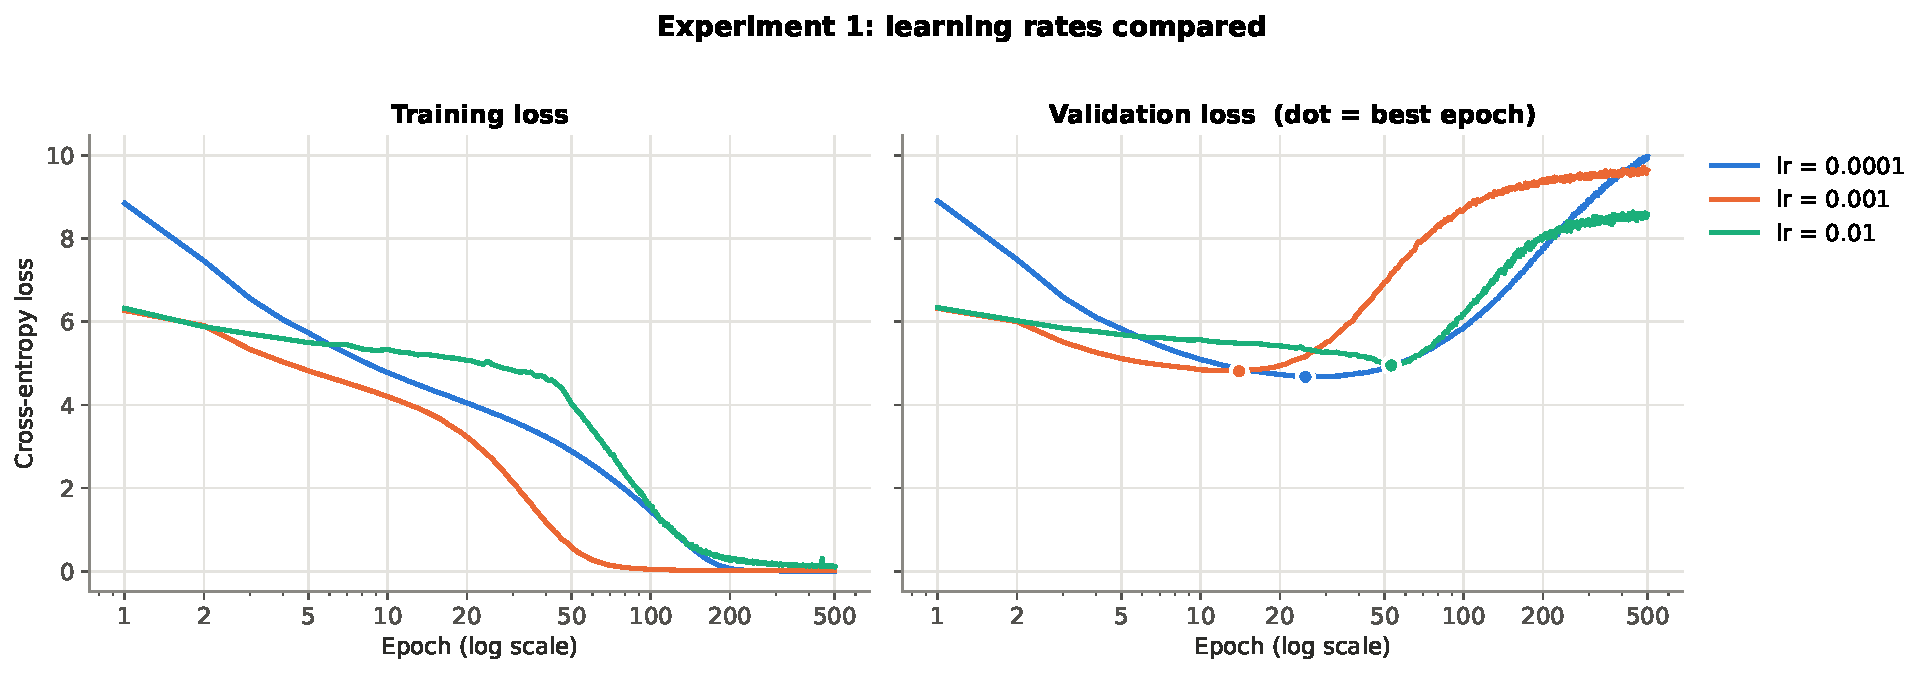
\includegraphics[width=\textwidth]{exp1_overlay.pdf}
  \caption{Experiment 1: all learning rates on common axes.}
\end{figure}

\begin{figure}[h]
  \centering
  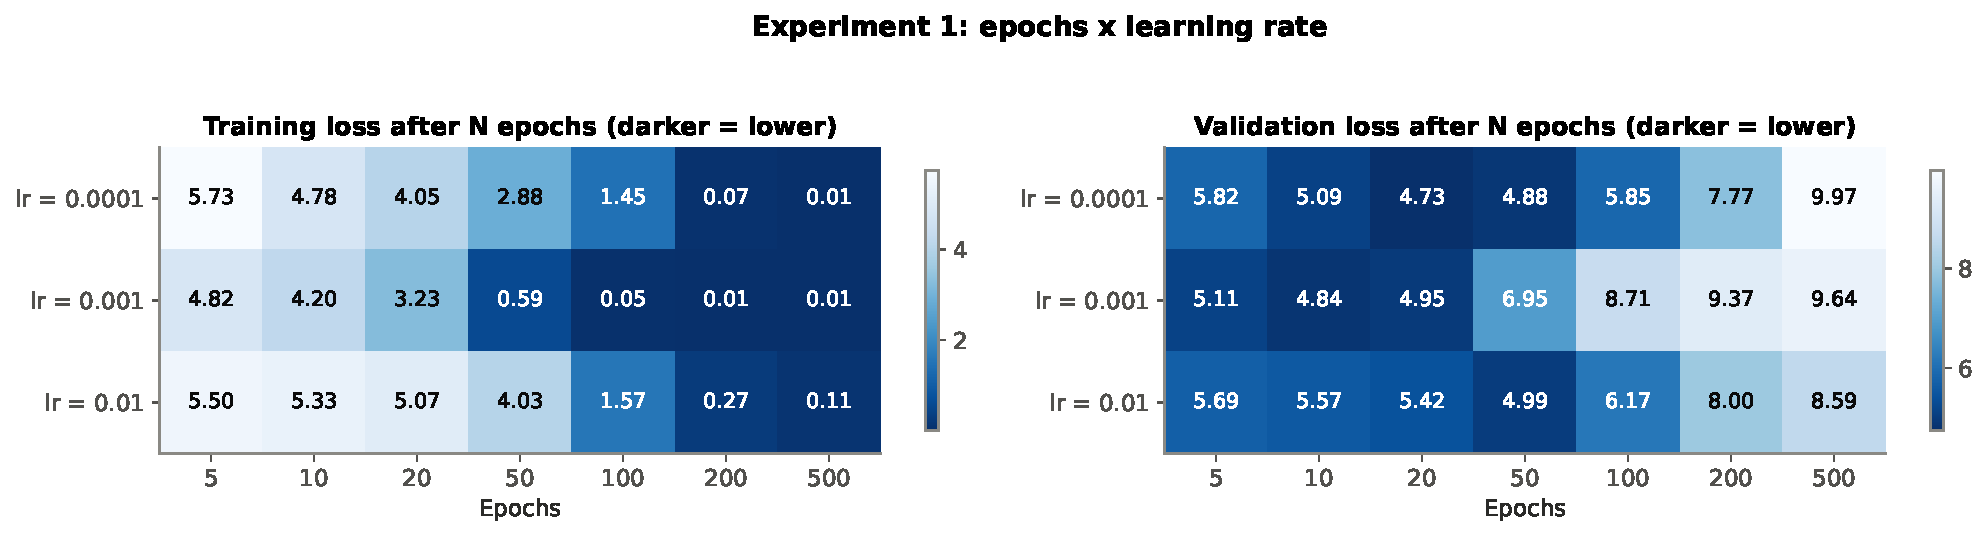
\includegraphics[width=\textwidth]{exp1_grid.pdf}
  \caption{Experiment 1: training and validation loss after $N$ epochs (darker is lower).}
\end{figure}

\begin{figure}[h]
  \centering
  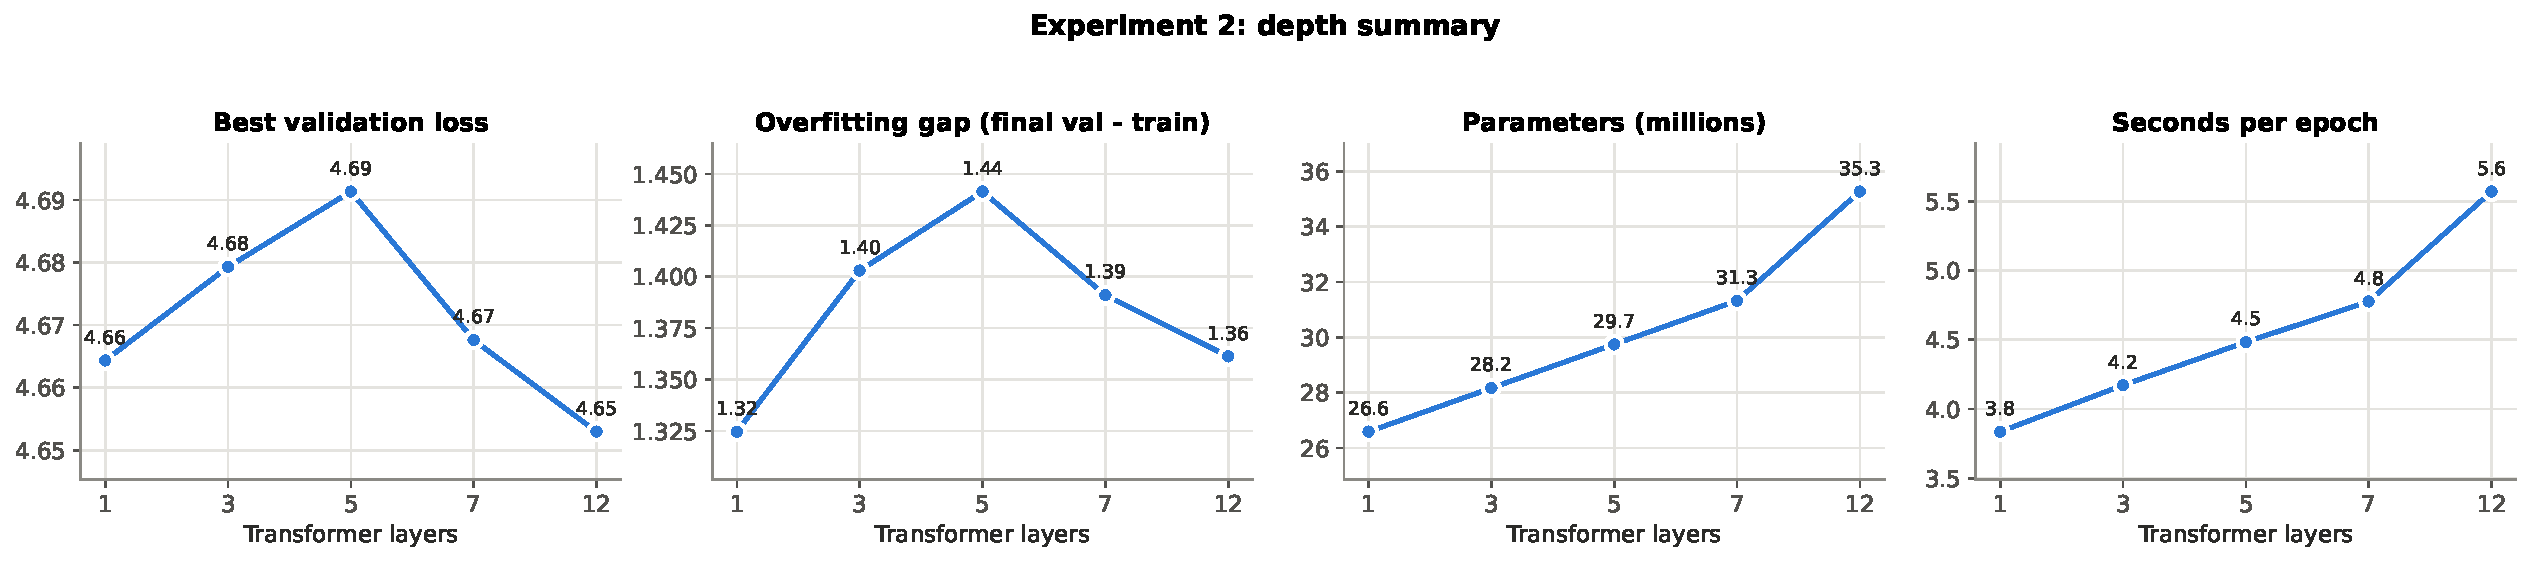
\includegraphics[width=\textwidth]{exp2_summary.pdf}
  \caption{Experiment 2 (seed 123): best validation loss, final generalisation gap, parameters and seconds per epoch against depth.}
\end{figure}

\begin{figure}[h]
  \centering
  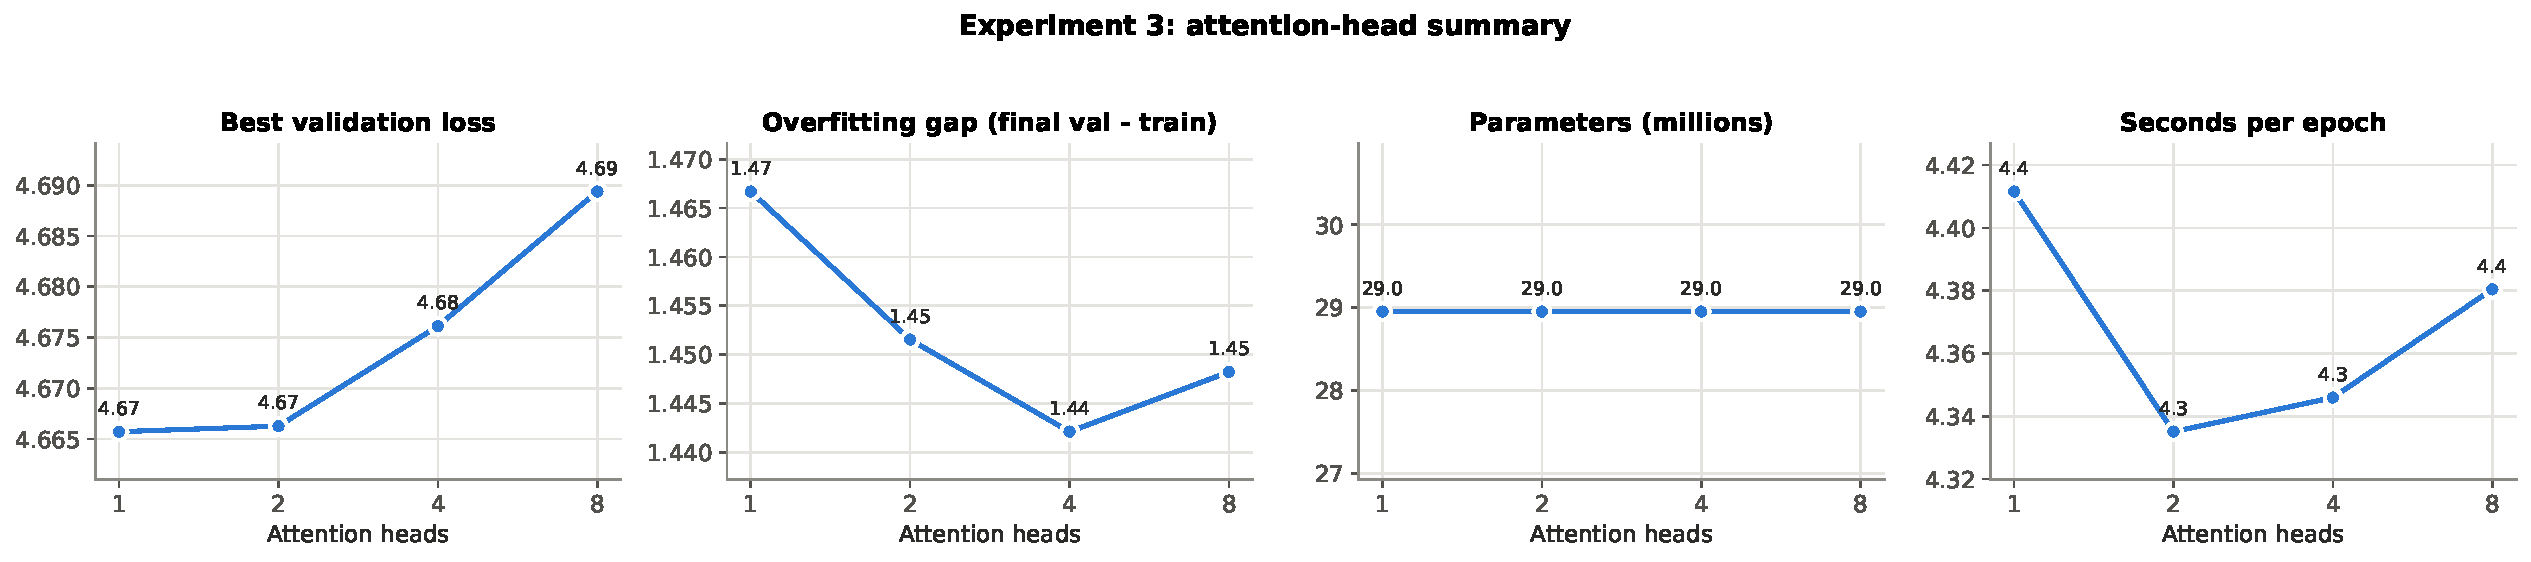
\includegraphics[width=\textwidth]{exp3_summary.pdf}
  \caption{Experiment 3 (seed 123): the same summary against the number of heads.}
\end{figure}

\begin{figure}[h]
  \centering
  \begin{subfigure}{0.49\textwidth}
    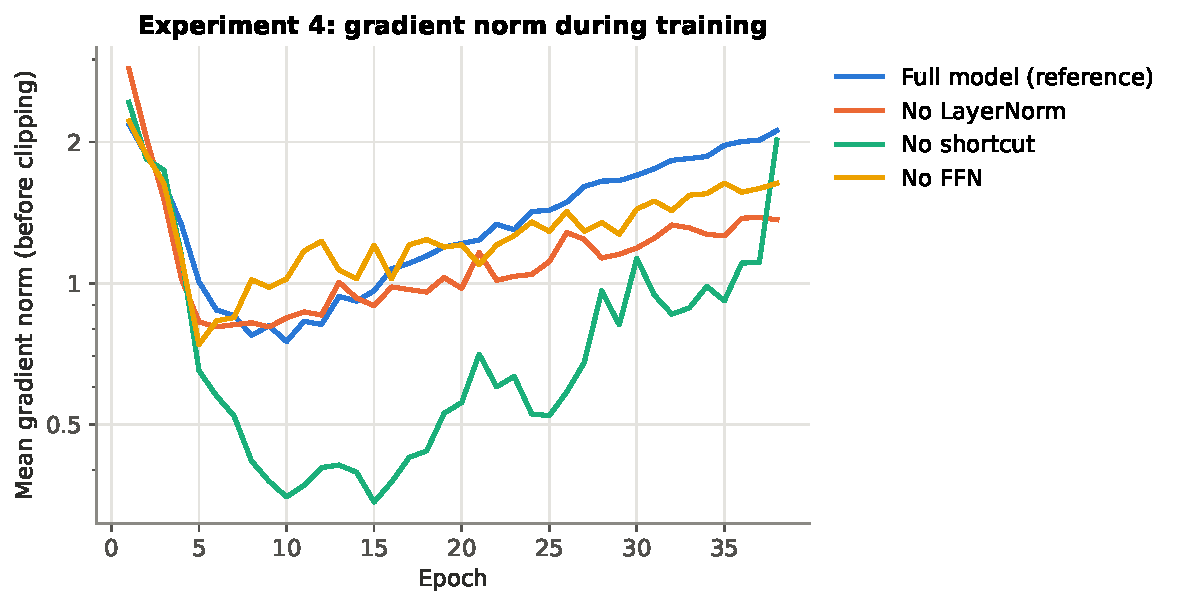
\includegraphics[width=\textwidth]{exp4_grad_norm.pdf}
    \caption{4 layers}
  \end{subfigure}\hfill
  \begin{subfigure}{0.49\textwidth}
    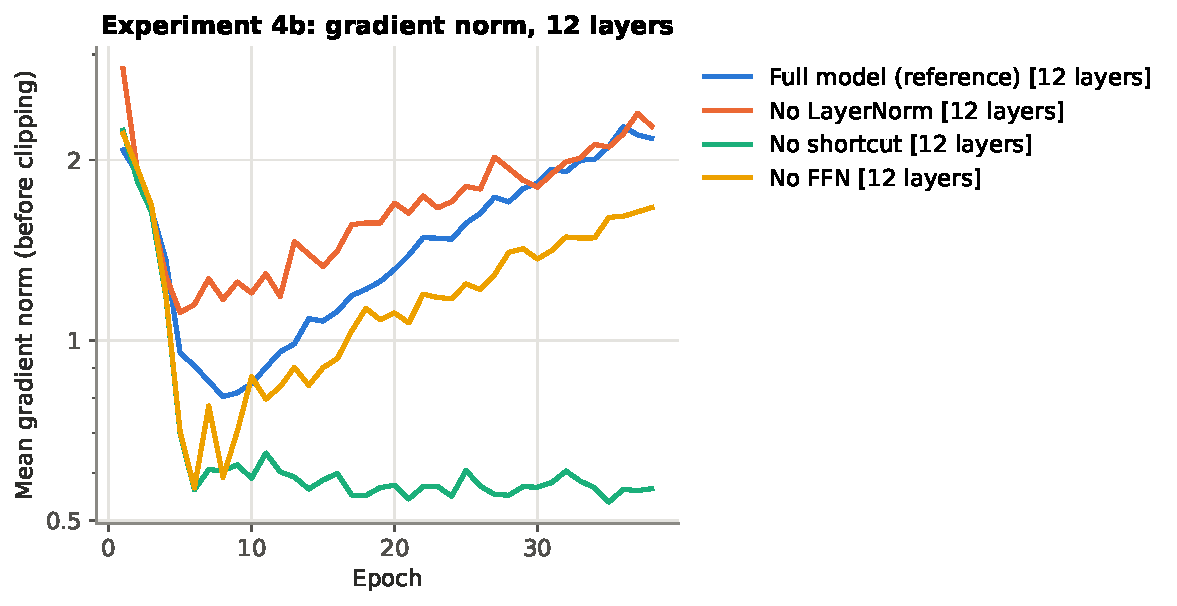
\includegraphics[width=\textwidth]{exp4b_grad_norm.pdf}
    \caption{12 layers}
  \end{subfigure}
  \caption{Gradient norm under the initial ablation protocol (LR $10^{-4}$).}
\end{figure}

\begin{figure}[h]
  \centering
  \begin{subfigure}{0.49\textwidth}
    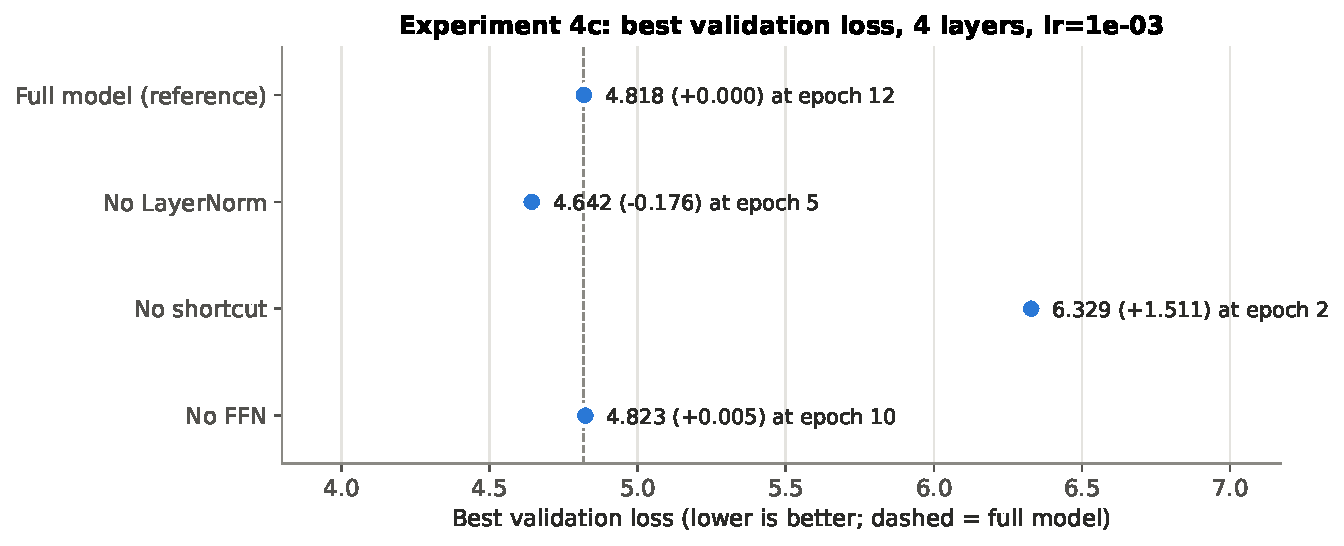
\includegraphics[width=\textwidth]{exp4c_L4_lr0.001_best.pdf}
    \caption{4 layers}
  \end{subfigure}\hfill
  \begin{subfigure}{0.49\textwidth}
    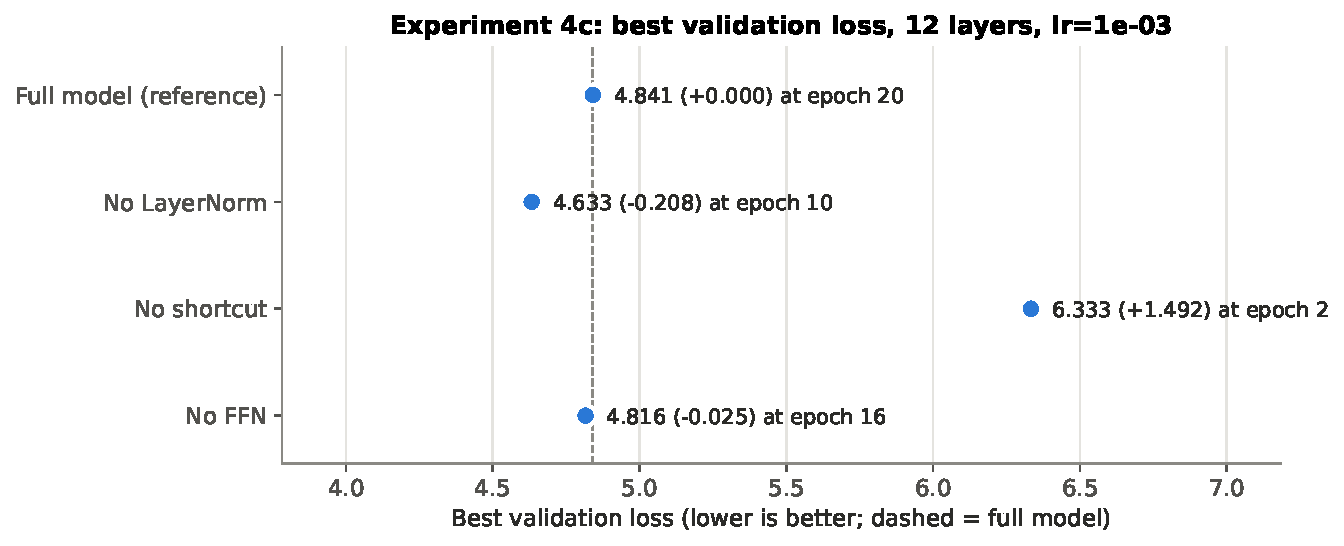
\includegraphics[width=\textwidth]{exp4c_L12_lr0.001_best.pdf}
    \caption{12 layers}
  \end{subfigure}
  \caption{Best validation loss of each ablation variant under the revised protocol (LR $10^{-3}$).}
\end{figure}

% ---------------------------------------------------------------------
\clearpage
\section{Complete Results}\label{app:results}
{\scriptsize
\setlength{\tabcolsep}{4pt}
\begin{longtable}{@{}lrrrrrrrrrrr@{}}
\caption{All 47 training runs (Colab T4 GPU). L = layers, H = heads, Ep.\ = epochs trained, Min.\ = minutes per run.}\label{tab:master}\\
\toprule
Run & L & H & LR & Seed & Ep. & Params (M) & Best val. & Best ep. & Final train & Final val. & Min. \\
\midrule
\endfirsthead
\toprule
Run & L & H & LR & Seed & Ep. & Params (M) & Best val. & Best ep. & Final train & Final val. & Min. \\
\midrule
\endhead
\bottomrule
\endfoot
\multicolumn{12}{@{}l}{\emph{Baseline}} \\
Baseline & 4 & 4 & $4\times10^{-4}$ & 123 & 20 & 28.95 & 4.616 & 10 & 2.473 & 4.973 & 1.4 \\
\midrule
\multicolumn{12}{@{}l}{\emph{Experiment 1: epochs and learning rate}} \\
LR 0.0001 & 4 & 4 & $1\times10^{-4}$ & 123 & 500 & 28.95 & 4.676 & 25 & 0.006 & 9.973 & 36.2 \\
LR 0.001 & 4 & 4 & $1\times10^{-3}$ & 123 & 500 & 28.95 & 4.809 & 14 & 0.009 & 9.645 & 35.8 \\
LR 0.01 & 4 & 4 & $1\times10^{-2}$ & 123 & 500 & 28.95 & 4.951 & 53 & 0.113 & 8.588 & 35.7 \\
\midrule
\multicolumn{12}{@{}l}{\emph{Experiment 2: layers (seed 123)}} \\
1 layer & 1 & 4 & $1\times10^{-4}$ & 123 & 38 & 26.59 & 4.664 & 30 & 3.369 & 4.694 & 2.4 \\
3 layers & 3 & 4 & $1\times10^{-4}$ & 123 & 38 & 28.16 & 4.679 & 25 & 3.337 & 4.740 & 2.6 \\
5 layers & 5 & 4 & $1\times10^{-4}$ & 123 & 38 & 29.74 & 4.691 & 30 & 3.311 & 4.753 & 2.8 \\
7 layers & 7 & 4 & $1\times10^{-4}$ & 123 & 38 & 31.32 & 4.668 & 29 & 3.308 & 4.699 & 3.0 \\
12 layers & 12 & 4 & $1\times10^{-4}$ & 123 & 38 & 35.27 & 4.653 & 29 & 3.335 & 4.696 & 3.5 \\
\midrule
\multicolumn{12}{@{}l}{\emph{Experiment 3: heads (seed 123)}} \\
1 head & 4 & 1 & $1\times10^{-4}$ & 123 & 38 & 28.95 & 4.666 & 29 & 3.271 & 4.738 & 2.8 \\
2 heads & 4 & 2 & $1\times10^{-4}$ & 123 & 38 & 28.95 & 4.666 & 29 & 3.278 & 4.730 & 2.7 \\
4 heads & 4 & 4 & $1\times10^{-4}$ & 123 & 38 & 28.95 & 4.676 & 25 & 3.299 & 4.741 & 2.8 \\
8 heads & 4 & 8 & $1\times10^{-4}$ & 123 & 38 & 28.95 & 4.689 & 25 & 3.306 & 4.754 & 2.8 \\
\midrule
\multicolumn{12}{@{}l}{\emph{Experiment 4: ablations, initial protocol}} \\
Full model & 4 & 4 & $1\times10^{-4}$ & 123 & 38 & 28.95 & 4.676 & 25 & 3.299 & 4.741 & 2.8 \\
No LayerNorm & 4 & 4 & $1\times10^{-4}$ & 123 & 38 & 28.95 & 4.627 & 37 & 3.710 & 4.630 & 2.7 \\
No shortcut & 4 & 4 & $1\times10^{-4}$ & 123 & 38 & 28.95 & 5.564 & 38 & 5.281 & 5.564 & 2.7 \\
No FFN & 4 & 4 & $1\times10^{-4}$ & 123 & 38 & 26.85 & 4.747 & 37 & 3.751 & 4.748 & 2.5 \\
Full model & 12 & 4 & $1\times10^{-4}$ & 123 & 38 & 35.27 & 4.653 & 29 & 3.335 & 4.696 & 3.5 \\
No LayerNorm & 12 & 4 & $1\times10^{-4}$ & 123 & 38 & 35.25 & 4.613 & 37 & 3.799 & 4.616 & 3.4 \\
No shortcut & 12 & 4 & $1\times10^{-4}$ & 123 & 38 & 35.27 & 6.316 & 11 & 6.274 & 6.342 & 3.4 \\
No FFN & 12 & 4 & $1\times10^{-4}$ & 123 & 38 & 28.95 & 4.824 & 37 & 4.047 & 4.831 & 2.9 \\
\midrule
\multicolumn{12}{@{}l}{\emph{Experiment 4: ablations, revised protocol}} \\
Full model & 4 & 4 & $1\times10^{-3}$ & 123 & 60 & 28.95 & 4.818 & 12 & 0.273 & 7.454 & 4.4 \\
No LayerNorm & 4 & 4 & $1\times10^{-3}$ & 123 & 60 & 28.95 & 4.642 & 5 & 0.403 & 7.476 & 4.3 \\
No shortcut & 4 & 4 & $1\times10^{-3}$ & 123 & 60 & 28.95 & 6.329 & 2 & 6.269 & 6.364 & 4.3 \\
No FFN & 4 & 4 & $1\times10^{-3}$ & 123 & 60 & 26.85 & 4.823 & 10 & 0.123 & 8.250 & 4.1 \\
Full model & 12 & 4 & $1\times10^{-3}$ & 123 & 60 & 35.27 & 4.841 & 20 & 0.320 & 7.171 & 5.6 \\
No LayerNorm & 12 & 4 & $1\times10^{-3}$ & 123 & 60 & 35.25 & 4.633 & 10 & 0.233 & 7.375 & 5.5 \\
No shortcut & 12 & 4 & $1\times10^{-3}$ & 123 & 60 & 35.27 & 6.333 & 2 & 6.269 & 6.363 & 5.5 \\
No FFN & 12 & 4 & $1\times10^{-3}$ & 123 & 60 & 28.95 & 4.816 & 16 & 0.536 & 7.340 & 4.7 \\
\midrule
\multicolumn{12}{@{}l}{\emph{Experiment 2: additional seeds}} \\
1 layers & 1 & 4 & $1\times10^{-4}$ & 42 & 38 & 26.59 & 4.658 & 32 & 3.385 & 4.675 & 2.5 \\
1 layers & 1 & 4 & $1\times10^{-4}$ & 7 & 38 & 26.59 & 4.666 & 30 & 3.370 & 4.706 & 2.5 \\
3 layers & 3 & 4 & $1\times10^{-4}$ & 42 & 38 & 28.16 & 4.669 & 30 & 3.328 & 4.711 & 2.7 \\
3 layers & 3 & 4 & $1\times10^{-4}$ & 7 & 38 & 28.16 & 4.659 & 31 & 3.329 & 4.716 & 2.7 \\
5 layers & 5 & 4 & $1\times10^{-4}$ & 42 & 38 & 29.74 & 4.682 & 28 & 3.305 & 4.733 & 2.9 \\
5 layers & 5 & 4 & $1\times10^{-4}$ & 7 & 38 & 29.74 & 4.664 & 27 & 3.310 & 4.717 & 2.9 \\
7 layers & 7 & 4 & $1\times10^{-4}$ & 42 & 38 & 31.32 & 4.655 & 27 & 3.306 & 4.699 & 3.1 \\
7 layers & 7 & 4 & $1\times10^{-4}$ & 7 & 38 & 31.32 & 4.662 & 27 & 3.311 & 4.714 & 3.1 \\
12 layers & 12 & 4 & $1\times10^{-4}$ & 42 & 38 & 35.27 & 4.659 & 31 & 3.316 & 4.701 & 3.6 \\
12 layers & 12 & 4 & $1\times10^{-4}$ & 7 & 38 & 35.27 & 4.643 & 27 & 3.330 & 4.681 & 3.6 \\
\midrule
\multicolumn{12}{@{}l}{\emph{Experiment 3: additional seeds}} \\
1 heads & 4 & 1 & $1\times10^{-4}$ & 42 & 38 & 28.95 & 4.663 & 28 & 3.298 & 4.720 & 2.8 \\
1 heads & 4 & 1 & $1\times10^{-4}$ & 7 & 38 & 28.95 & 4.661 & 28 & 3.274 & 4.713 & 2.9 \\
2 heads & 4 & 2 & $1\times10^{-4}$ & 42 & 38 & 28.95 & 4.670 & 27 & 3.300 & 4.717 & 2.8 \\
2 heads & 4 & 2 & $1\times10^{-4}$ & 7 & 38 & 28.95 & 4.663 & 28 & 3.301 & 4.704 & 2.8 \\
4 heads & 4 & 4 & $1\times10^{-4}$ & 42 & 38 & 28.95 & 4.677 & 28 & 3.299 & 4.722 & 2.8 \\
4 heads & 4 & 4 & $1\times10^{-4}$ & 7 & 38 & 28.95 & 4.682 & 27 & 3.312 & 4.724 & 2.8 \\
8 heads & 4 & 8 & $1\times10^{-4}$ & 42 & 38 & 28.95 & 4.678 & 27 & 3.309 & 4.736 & 2.8 \\
8 heads & 4 & 8 & $1\times10^{-4}$ & 7 & 38 & 28.95 & 4.679 & 28 & 3.313 & 4.750 & 2.8 \\
\end{longtable}

}

\end{document}
